\documentclass[runningheads]{llncs}

\usepackage[T1]{fontenc}
\usepackage{graphicx}
\usepackage{svg}
\usepackage[ngerman]{babel}
\usepackage[utf8]{inputenc}
\usepackage[babel, german=guillemets]{csquotes}
\usepackage{mathtools}
\usepackage{xfrac}
\usepackage{multirow}
\usepackage{multicol}
\usepackage[hidelinks]{hyperref}
\usepackage{color}
\usepackage[nolist]{acronym}
\usepackage{listings}
\usepackage{tabularx}
\usepackage{makecell}
\usepackage{pifont}
\renewcommand\UrlFont{\color{blue}\rmfamily}
\newcommand{\cmark}{\ding{51}}

\graphicspath{ {./img/} }

\begin{document}

\title{Apples „Wo ist“ Dienst – Funktionsweise und Missbrauchspotential}


\author{Lukas Panni\inst{1}}

\authorrunning{L. Panni}
\institute{Hochschule Karlsruhe, Karlsruhe}

\maketitle              % typeset the header of the contribution

\begin{abstract}
Apples „Wo ist“ Dienst ist aufgrund der großen Verbreitung von Apple-Geräten und fehlender Schutzmaßnahmen ein interessantes Ziel für Angreifer und bietet großes Missbrauchspotential.

Als Crowdsourced-Tracking-Dienst verwendet „Wo ist“ zur Lokalisierung verlorener Geräte andere Apple-Geräte in der Umgebung.
Verlorene Geräte senden regelmäßig Daten über \ac{BLE} an alle Geräte der Umgebung, welche den Standort bestimmen und Ende-zu-Ende verschlüsselt an Apple übertragen.
Besitzer verlorener Geräte können die Standortdaten von Apples Servern abrufen, entschlüsseln und das Gerät lokalisieren.

Die vorliegende Arbeit beschreibt die Funktionsweise des „Wo ist“ Dienstes und zeigt, welche Maßnahmen getroffen werden, um die Privatsphäre der Nutzer zu schützen.
Weiterhin werden konkrete Missbrauchsszenarien aufgezeigt, gegen welche die ergriffenen Sicherheitsmaßnahmen nur unzureichend schützen.
Basierend darauf werden Maßnahmen vorgeschlagen, wie Apple und die Nutzer des Dienstes den Missbrauch in einigen Fällen verhindern können.
Jedoch kann ohne eine umfassende Anpassung auch mit zusätzlichen Maßnahmen nicht jeder Missbrauch komplett ausgeschlossen werden.
\keywords{ Apple \and Bluetooth \and Privatsphäre \and Tracking }
\end{abstract}

\begin{acronym}[AAAAA]

    \acro{API}[API]{Application Programming Interface}
    \acro{AES}[AES]{Advanced Encryption Standard}
    \acro{BLE}[BLE]{Bluetooth Low Energy}
    \acro{DSGVO}[DSGVO]{Datenschutzgrundverordnung}
    \acro{DOS}[DoS]{Denial of Service}
    \acro{ECC}[ECC]{Elliptic Curve Cryptography}
    \acro{ECDH}[ECDH]{Elliptic Curve Diffie-Hellman}
    \acro{GCM}[GCM]{Galois/Counter Mode}
    \acro{GPS}[GPS]{Global Positioning System}
    \acro{IOT}[IoT]{Internet of Things}
    \acro{KDF}[KDF]{Key Derivation Function}
    \acro{MAC}[MAC]{Media Access Control}
    \acro{MBK}[MBK]{Master Beacon Key}
    \acro{MITM}[MitM]{Man-in-the-Middle}
    \acro{MSB}[MSB]{Most Significant Bit}
    \acro{SHA}[SHA]{Secure Hash Algorithm}
    \acro{TLS}[TLS]{Transport-Layer Security}
    
\end{acronym}


\section{Einleitung}
\subsection{Motivation}
% TODO: Motivation

\cite{Spec_BLE_5.3}
\newpage
\section{Grundlagen}
\label{sec:grundlagen}

Die folgenden Abschnitte dienen als kurze Einführung zu den technologischen Grundlagen von Apples „Wo ist“ Dienst.
Dazu werden insbesondere der Standard zu kabellosen Kurzstreckenkommunikation \ac{BLE} und die asymmetrische Verschlüsselung auf Basis elliptischer Kurven, auch \ac{ECC}, vorgestellt.

\subsection{\ac{BLE}}
\label{sec:ble}
Für die Erklärung der Funktionsweise ist insbesondere das \ac{BLE}-Advertising relevant.
Der Standard für \ac{BLE} ist ein Teil des Bluetooth Standards und auf Kurzstreckenkommunikation bei geringem Energieverbrauch ausgelegt.
Das Advertising wird dazu verwendet, das Gerät für andere Geräte in der Umgebung auffindbar zu machen.
Dazu werden Advertisement-Pakete im Abstand von einem sogenannten \textit{Advertising-Intervall} gesendet \cite{Spec_BLE_5.3}.
Für das Advertising stellt der \ac{BLE}-Standard drei der 40 verfügbaren Kanäle im Frequenzbereich von 2,4 GHz bis 2,4835 GHz zur Verfügung.
Jedes Advertisement-Paket wird nacheinander, mit einer zufälligen Verzögerung zur Kollisionsvermeidung, in jedem der drei Kanäle gesendet.
Das minimale Advertising-Intervall beträgt 20 Millisekunden, das maximale 10,24 Sekunden \cite{Spec_BLE_5.3}.
Je länger das Intervall, desto geringer ist der Energieverbrauch des Geräts, das die Advertisement-Pakete sendet.
Allerdings leidet die Auffindbarkeit unter langen Intervallen.
Apple verwendet für den „Wo ist“ Dienst als Kompromiss zwischen optimaler Auffindbarkeit und minimalem Energieverbrauch ein Advertising-Intervall von zwei Sekunden \cite{Apple_FindMySpec}.


Der \ac{BLE}-Standard erlaubt es, beliebige Daten in einem Advertisement-Paket zu versenden, sofern der Typ des Pakets als \textit{manufacturer-specific-data} festgelegt wird.
In diesem Fall kann das Paket 27 Byte Nutzdaten enthalten \cite{Spec_BLE_5.3}.
Da Apple für andere Dienste, wie beispielsweise AirDrop, ebenfalls \ac{BLE} nutzt, kommt ein proprietäres Format für die Nutzdaten zum Einsatz \cite{Heinrich_FindMy}.
Das genaue Format für den „Wo ist“ Dienst wird in \autoref{fig:apple_advertising} vorgestellt.

Um Advertisement-Pakete zu empfangen, müssen die Advertising-Kanäle abgehört werden.
Dazu wechseln die Geräte jeweils auf einen der Kanäle und erfassen Advertisement-Pakete für eine definierte Zeit.
Anschließend wird nach einer Wartezeit auf den nächsten Kanal gewechselt \cite{Spec_BLE_5.3}.
Wie häufig und wie lange Apple-Geräte im Hintergrund die Kanäle nach Advertisement-Paketen anderer Apple-Geräte abhören, ist nicht bekannt.

\section{\ac{ECC}}
\label{sec:ecc}
Auf elliptischen Kurven basierende Kryptografieverfahren gehören zu den asymmetrischen Verschlüsselungsverfahren.
Asymmetrisch sind alle Verfahren, welche für die Verschlüsselung und die Entschlüsselung zwei verschiedene Schlüssel verwenden.
Der für die Verschlüsselung verwendete Schlüssel muss dabei nicht geheim gehalten werden, da verschlüsselte Nachrichten mit diesem nicht entschlüsselt werden können.
Der Schlüssel kann öffentlich zugänglich gemacht werden.
Daher heißt der Verschlüsselungsschlüssel auch öffentlicher Schlüssel oder \textit{public key}.
Der Entschlüsselungsschlüssel, auch privater Schlüssel oder \textit{private key} genannt, muss hingegen geheim gehalten werden \cite[S. 173ff.]{Krypto}.

Die asymmetrische Verschlüsselung löst somit das Problem des Schlüsselaustauschs bei symmetrischen Verschlüsselungsverfahren, bei denen nur ein Schlüssel existiert, welcher geheim gehalten werden muss.
Jedoch sind asymmetrische Verfahren meist rechenintensiver und damit langsamer als symmetrische Verfahren mit vergleichbarem Sicherheitsniveau.
Oft werden deshalb Hybride Verfahren verwendet \cite[S. 178f.]{Krypto}.
Auch für die Verschlüsselung der Standortdaten in Apples „Wo ist“ Dienst wird ein hybrides Verfahren verwendet, welches in \autoref{sec:Funktionsweise_FindMy} näher erläutert wird.

Für den „Wo ist“ Dienst wird \ac{ECC} verwendet.
Verfahren auf Basis von elliptischen Kurven erreichen ein vergleichbares Sicherheitsniveau mit kürzeren Schlüsseln als andere asymmetrische Verfahren \cite[S. 273.]{Krypto}.
Dieser Vorteil wird ausgenutzt, damit der öffentliche Schlüssel in \ac{BLE} Advertisement-Paketen übertragen werden kann.
Meist kommen standardisierte elliptische Kurven zum Einsatz, Apple nutzt beispielsweise die NIST P-224 Kurve \cite{Heinrich_FindMy}.
Jede Kurve wird durch eine Primzahl, zwei Kurvenkoeffizenten und einen primitiven Punkt auf der Kurve definiert.
Der private Schlüssel ist eine zufällige ganze Zahl.
Durch die Multiplikation des privaten Schlüssels mit dem primitiven Punkt wird der öffentliche Schlüssel als Punkt auf der Kurve berechnet.
Der öffentliche Schlüssel wird in Form der X und Y Koordinate des Punktes angegeben.
Weiterhin lässt sich der öffentliche Schlüssel in der Praxis auf eine Koordinate reduzieren \cite[S. 284f.]{Krypto}.

Schlüssel werden oft nur für einen begrenzten Zeitraum verwendet, wodurch sich die Sicherheit erhöhen kann \cite[S. 378f.]{Krypto}.
Wenn der Schlüssel für die Verschlüsselung der Standortdaten regelmäßig gewechselt wird, kann ein Angreifer, auch wenn er einen Schlüssel erlangt, nur die Standortdaten aus einer begrenzten Zeit abrufen.
Weiterhin kann die Zuordnung von öffentlichem Schlüssel zu einem Gerät durch häufiges Wechseln der Schlüssel erschwert werden.
\ac{KDF} können genutzt werden, um aus bestehenden Schlüsseln und einer Zusatzinformation neue Schlüssel zu erzeugen.
Dabei kann jeder, der den Schlüssel und die Zusatzinformation kennt, neue Schlüssel ableiten \cite[S. 378ff.]{Krypto}.
Im „Wo ist“ Dienst wird eine \ac{KDF} genutzt, um aus einem geheimen Schlüssel und einem Zähler regelmäßig neue Schlüsselpaare abzuleiten \cite{Heinrich_FindMy}.

\section{Crowdsourced-Tracking: Funktionsweise}
\label{sec:Funktionsweise}

Mit der Einführung ihres ersten \ac{BLE}-Trackers hat die Firma Tile 2013 das Konzept eines \ac{BLE}-basierten Tracking-Systems populär gemacht.
Wie viele konkurrierende Systeme, darunter Apples „Wo ist?“ Dienst, setzt auch Tile auf crowdsourcing zur Bestimmung der Position verlorener Gegenstände \cite{Weller_BLE_Finders}.
Die grundlegende Funktion dieser Systeme ist jeweils identisch und in \autoref{fig:tracker_allgemein} gezeigt: Ein zu findendes Gerät \textit{a)} sendet periodisch \ac{BLE}-Advertisements, die von Smartphones in der Nähe \textit{b)}, welche am entsprechenden System teilnehmen, empfangen werden können \textit{(1)}.
Das zu findende Gerät ist dabei entweder ein Endgerät wie ein Smartphone oder ein Tablet, oder ein spezieller, batteriebetriebener, sogenannter Tracker.
Solche Tracker können an anderen Gegenstände befestigt werden, sodass diese bei Verlust ebenfalls gefunden werden können.
Die Empfänger der \ac{BLE}-Advertisements können ihre Position über das \ac{GPS} bestimmen und diese zusammen mit einer ID, welche das zu findende Gerät identifiziert, an einen Server übermitteln \textit{(2)}.
Der Besitzer des verlorenen Geräts \textit{c)} kann die Position seines Geräts vom Server abrufen \textit{(3)} \cite{Garg_Secure_Tracker}.
Das Funktionsprinzip ist dementsprechend vergleichsweise einfach.
\begin{figure}[ht]
    \centering 
    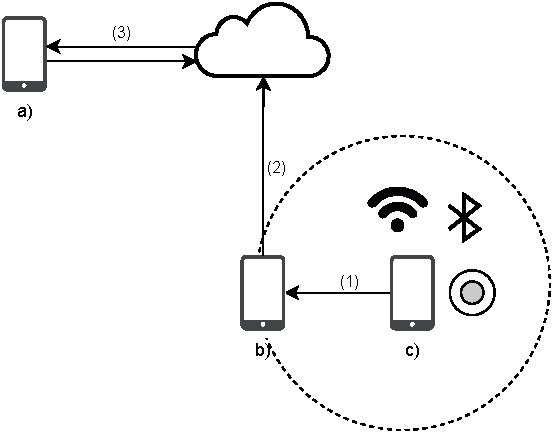
\includegraphics[width=0.9\textwidth]{BLE_Tracker_allgemein.pdf}
    \caption{Allgemeine Funktionsweise des Crowdsourced-Tracking mit \ac{BLE}.}
    \label{fig:tracker_allgemein}
\end{figure}
Qualität und Nützlichkeit für die Nutzer eines solchen Dienstes hängt aber stark von der Anzahl der Nutzer ab.
Die Position eines verlorenen Geräts kann nur vom Tracking-Dienst abgerufen werden, wenn ein Nutzer des gleichen Dienstes ein \ac{BLE}-Advertisement des verlorenen Geräts empfangen und die Position an den Dienst übermittelt hat.
Je mehr Nutzer ein Dienst hat, desto größer die Wahrscheinlichkeit, dass sich ein Nutzer vor kurzem in der Nähe des verlorenen Geräts befand und desto größer die Wahrscheinlichkeit, das verlorene Gerät zu finden.


In allen untersuchten Systemen konnten Weller \textit{et al.} \cite{Weller_BLE_Finders} und Garg \textit{et al.} \cite{Garg_Secure_Tracker} unabhängig voneinander verschiedene Schwachstellen finden, die sowohl Privatsphäre als auch Sicherheit betreffen.
Unter anderem übermittelten einige Dienste die Positionsdaten unverschlüsselt und erlaubten das unberechtigte Abrufen von personenbezogenen Daten über die Backends der Dienste.
Auch zum Veröffentlichungszeitpunkt der Arbeit von Weller \textit{et al.} \cite{Weller_BLE_Finders} waren nicht alle der erkannten Schwachstellen behoben.
Außerdem bot keiner der von Garg \textit{et al.} \cite{Garg_Secure_Tracker} untersuchten Dienste ausreichend Schutz vor dem Melden falscher Positionsdaten.


\subsection{Funktionsweise des „Wo ist?“ Dienstes im Detail}
\label{sec:Funktionsweise_FindMy}
Auf seiner Informationsseite über den „Wo ist?“ Dienst gibt Apple an: „Geräte in der Nähe senden den Standort [...] sicher an iCloud weiter [...]. Zum Schutz der Privatsphäre passiert das alles anonym und verschlüsselt“ \cite{Apple_WoIst}.
Apple erhebt demnach den Anspruch einen Dienst anzubieten, der nicht nur sicherer, sondern auch besser für die Privatsphäre der Nutzer ist als die Dienste der Konkurrenz.
Vergangene Untersuchungen haben allerdings bereits gezeigt, dass auch Apples Dienst einige Schwachstellen aufweist \cite{Heinrich_FindMy,Tonetto_FindMy}.
Diese Schwachstellen werden in \autoref{sec:Missbrauch} wieder aufgegriffen.

Der vermutlich größte Vorteil des Dienstes liegt vermutlich aber in der großen Zahl der Geräte, welche aktiv die Positionsdaten verlorener Geräte sammeln.
Laut Apple nehmen „hunderte[n] Millionen iPhone, iPad und Mac Geräte[n]“ \cite{Apple_WoIst} am „Wo ist?“ Dienst teil.
Der größte Konkurrent Tile hatte im Jahr 2021 laut der bekannten Gadget-Review Webseite \textit{Pocket-Lint} 40 Millionen Nutzer und kann damit für die Lokalisierung auf ein deutlich kleineres Netzwerk zurückgreifen als Apple \cite{Tile_Network}.


Auf Basis des Reverse-Engineering des „Wo ist?“ Dienstes von Heinrich \textit{et al.} in \cite{Heinrich_FindMy} und der Spezifikation für Drittanbieter \cite{Apple_FindMySpec} wird im Folgenden die grundlegende Funktionsweise des Dienstes erläutert.
Dabei wird insbesondere darauf eingegangen, welche Maßnahmen Apple ergreift um Sicherheit und Privatsphäre der Nutzer besser zu schützen als die konkurrierenden Dienste. 

In der Spezifikation werden folgende vier Rollen definiert \cite{Apple_FindMySpec}:
\begin{itemize}
    \item \textbf{Owner Device}: Alle Geräte, in denen die Apple-ID des Besitzers hinterlegt ist.
    \item \textbf{Accessory}: Das zu findende Gerät.
    \item \textbf{Find My network}: Die Menge aller Apple-Geräte, mit aktivierter „Wo ist?“ Funktion. Einzelne Geräte werden jeweils als \textbf{Finder Device} bezeichnet.
    \item \textbf{Apple Server}: Server der die Standortinformationen speichert.
\end{itemize}
\autoref{fig:findMy_roles} zeigt die Rollen, deren Beziehungen und die jeweiligen Aufgaben wie in der Spezifikation angegeben.
\begin{figure}
    \centering
    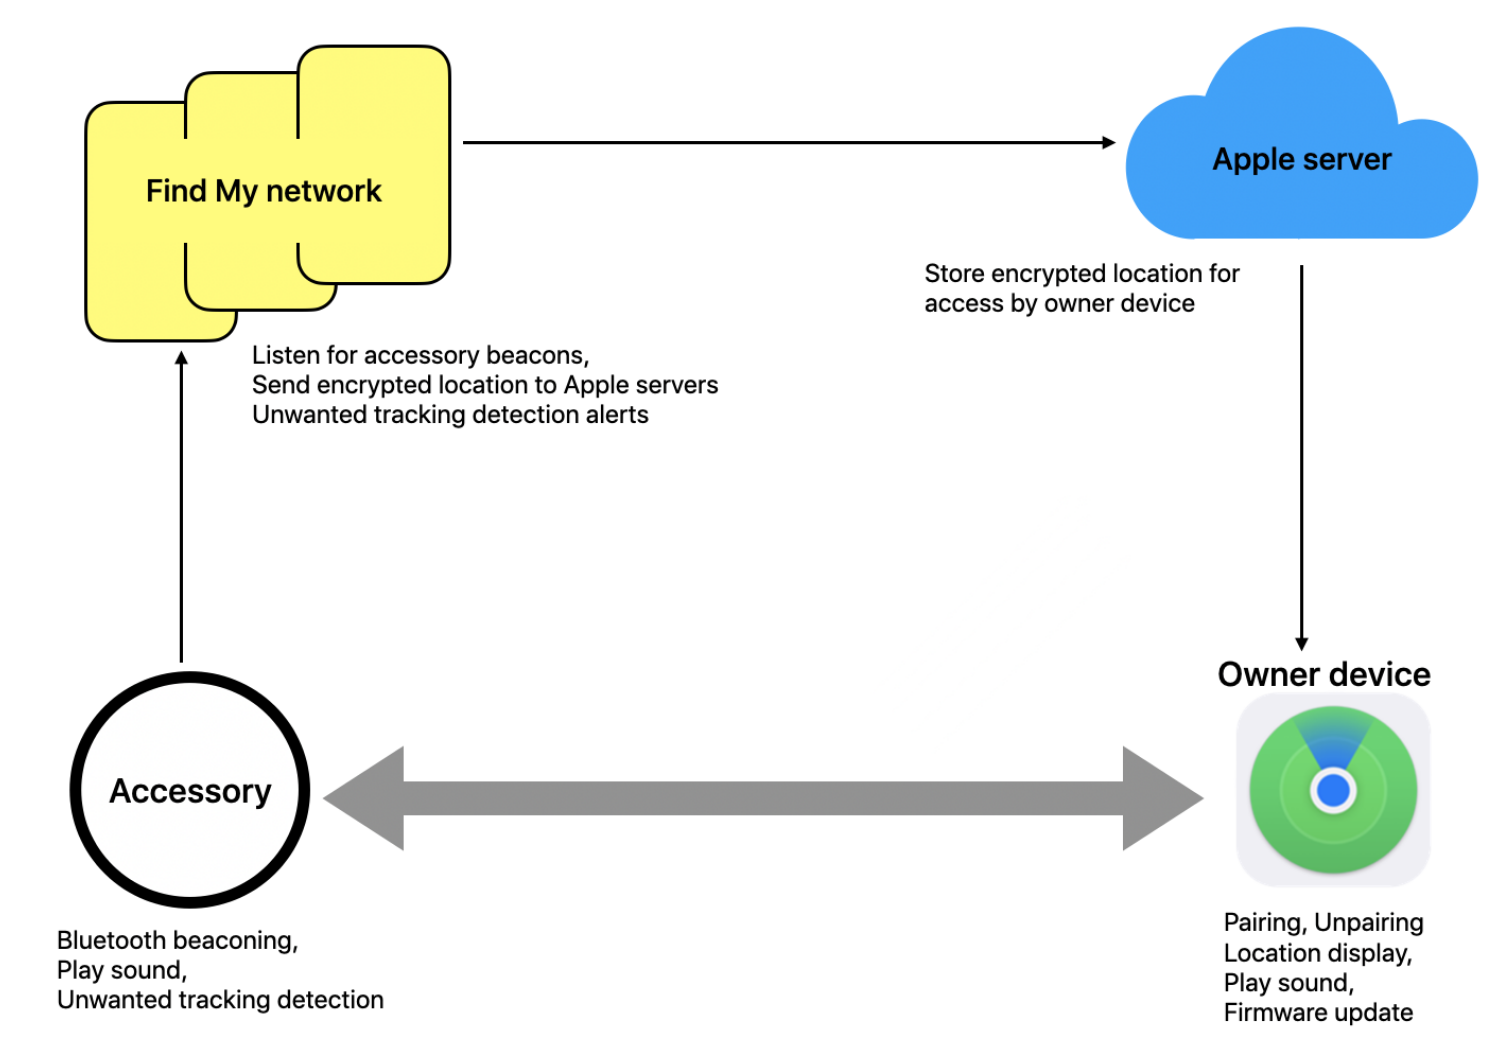
\includegraphics[width=0.9\textwidth]{findMy_roles}
    \caption{Rollen im „Wo ist?“ Dienst \cite{Apple_FindMySpec}.}
    \label{fig:findMy_roles}
\end{figure}
Apple erlaubt seit April 2021 auch Drittanbietern die Nutzung des „Wo ist?“ Netzwerks um die eigenen Produkte zu finden \cite{Apple_FindMy3rdParty}.
Da die Spezifikation speziell für Drittanbieter erstellt wurde, wird das zu findende Gerät als \textit{Accessory} bezeichnet.
In der folgenden Beschreibung wird jedoch der Begriff \textit{Lost Device} verwendet, der auch von Heinrich \textit{et al.} \cite{Heinrich_FindMy} verwendet wird und sowohl Produkte von Drittanbietern als auch von Apple abdeckt.
Das zu findende Gerät muss mit der Apple-ID des Besitzers verbunden sein, um gefunden werden zu können.
Drittanbieter Geräte und AirTags müssen dazu vor der ersten Verwendung über einen Pairing-Prozess mit einem Apple-Gerät verbunden werden \cite{Apple_FindMySpec}.

\subsubsection{Kryptografie}
\label{sec:Kryptografie}

Um bessere Sicherheit und Privatsphäre als die Konkurrenz zu bieten, setzt Apple auf asymmetrische \ac{ECC} Verschlüsselung.
Standortdaten werden immer Ende-zu-Ende verschlüsselt, sodass potenzielle Angreifer die Positionen der Nutzer nicht verfolgen können, sollten sie an Standortdaten gelangen.
Durch den verwendeten Prozess zur Verschlüsselung kann auch Apple selbst nicht auf die Standortdaten zugreifen.
Nur der Besitzer des Geräts kann die Standortdaten zur Lokalisierung des Geräts entschlüsseln \cite{Greenberg_FindMyCrypto}.


Jedes Owner Device erstellt zunächst den sogenannten \textit{Master Beacon Key}, bestehend aus einem \ac{ECC} Schlüsselpaar und einem symmetrischen Schlüssel.
Diese Schlüssel werden über den iCloud Dienst zwischen allen Geräten mit der gleichen Apple-ID synchronisiert.
Um die Schlüssel bei der Synchronisierung zu schützen, werden sie mit einem symmetrischen Schlüssel, aus der als sicher geltenden iCloud Keychain, verschlüsselt \cite{Heinrich_FindMy,Afonin_iCloudKeychain}.
Der private Schlüssel des \ac{ECC}-Schlüssels sowie der symmetrische Schlüssel des Master Beacon Keys müssen geheim bleiben.
Auch der öffentliche Teil des \ac{ECC}-Schlüssels im Master Beacon Key, wird nie über \ac{BLE} übertragen.
Stattdessen wird der Master Beacon Key verwendet, um temporär gültige Schlüssel abzuleiten, die im \ac{BLE}-Advertising übertragen werden können.
Für die Ableitung dieser sogenannten \textit{Advertising Keys} wird die ANSI X9.63-\ac{KDF} verwendet \cite{Apple_FindMySpec}.
Aus einem im \ac{BLE}-Advertising übertragenen öffentlichen Schlüssel kann somit, ohne Kenntnis des Master Beacon Keys, der nächste öffentliche Schlüssel nicht abgeleitet werden.
Durch regelmäßiges Wechseln des verwendeten Avertising Keys wird es einem Angreifer erschwert, ein Lost Device anhand der im Advertising übertragenen Daten zu verfolgen.
Da für die Verschlüsselung der Standortdaten nur die X-Koordinate des öffentlichen Schlüssels benötigt wird, kann auf die Übertragung der Y-Koordinate verzichtet werden \cite{Heinrich_FindMy}.

Die Verschlüsselung der Standortdaten erfolgt auf dem Finder Device mit dem \ac{AES}-Algorithmus im \ac{GCM}-Modus.
Aus dem, vom Finder Device empfangenen, Advertising Key wird ein temporäres \ac{ECC}-Schlüsselpaar generiert, aus welchem über einen \ac{ECDH} Schlüsselaustauch ein geteiltes Geheimnis generiert und durch die Anwendung der ANSI X9.63-\ac{KDF} ein symmetrischer Schlüssel abgeleitet wird.
Der Schlüsselaustausch verwendet den privaten Teil des temporären \ac{ECC}-Schlüssels und den öffentlichen Teil des empfangenen Advertising Keys.
Von diesem werden die ersten 16 Byte als Schlüssel für den \ac{AES}-Algorithmus und die folgenden 16 Byte als Initialisierungsvektor verwendet \cite{Heinrich_FindMy}.
Durch die Ausführung der Verschlüsselung auf dem Finder Device, kann die Batterie des Lost Devices geschont werden und die Lokalisierung verlorener Geräte bleibt länger möglich.
Insbesondere bei AirTags oder Produkten von Drittanbietern kann das hilfreich sein, da diese Geräte, eine im Vergleich zu einem iPhone oder iPad, sehr geringe Batteriekapazität haben.
Die kryptografischen Funktionen könnten den Stromverbrauch der Geräte deutlich erhöhen, wenn bei jedem Kontakt mit einem Finder-Device dieser komplexe Verschlüsselungsprozess ablaufen muss.
Durch die Verschlüsselung auf den Finder Devices müssen die Lost Devices nur alle 15 Minuten einen neuen Schlüssel ableiten, was durch die geringere Zahl der Operationen eine deutlich geringere Belastung für die Batterie darstellt.


Für die Entschlüsselung kann das geteilte Geheimnis über den \ac{ECDH} Schlüsselaustausch mit dem öffentlichen Teil des temporären Schlüssels und dem privaten Teil des Advertising Keys berechnet werden.
Der symmetrische Schlüssel entsteht wieder durch die Anwendung der ANSI X9.63-\ac{KDF} auf das geteilte Geheimnis.
Damit ist sichergestellt, dass die verschlüsselten Daten nur vom Besitzer entschlüsselt werden können.
Dieser kann die für das Advertisement verwendeten Schlüsselpaare unabhängig vom verlorenen Gerät aus dem Master Beacon Key ableiten und hat somit Zugriff auf die privaten Schlüssel.
Der öffentliche Teil des temporären Schlüssels und ein \ac{SHA}-256 Hash des verwendeten Advertisement Keys wird mit den verschlüsselten Daten auf Apples Server hochgeladen.
Der Besitzer kann diese Daten abrufen und aus der Kombination des öffentlichen temporären Schlüssels und dem privaten Advertisement Keys das geteilte Geheimnis und somit den symmetrischen Schlüssel berechnen \cite{Heinrich_FindMy}.

Da Geräte ohne Internetverbindung, wie zum Beispiel AirTags oder andere Geräte von Drittanbietern, die Master Beacon Keys nicht über die iCloud Synchronisation erhalten können, müssen diese Geräte auf andere Weise an einen initialen Schlüssel kommen.
% TODO: Schlüsselaushandlung, Infos aus Spec

\subsubsection{Ablauf beim Verlust eines Geräts}
\label{sec:Verlust}

Alle Apple Geräte mit aktivierter Bluetooth-Funktion, die für das Finden durch den „Wo ist?“ Dienst angemeldet sind, senden periodisch, in der Regel im Advertising Intervall von 2 s \ac{BLE}-Advertisements.
Die im Advertisement enthaltenen Daten unterscheiden sich jedoch abhängig vom Zustand des Geräts.
iPhones, iPads und MacBooks mit Internetverbindung und alle unterstützen Geräte mit einer aktiven \ac{BLE}-Verbindung mit einem Owner Device, gelten nicht als Lost Device und senden deshalb nur die ersten fünf Bytes des öffentlichen Advertisement Keys.
Das Advertisement erfolgt vermutlich um erkennen zu können, wenn ein Gerät in der Nähe die Verbindung verliert.
Die ersten fünf Byte des öffentlichen Schlüssels sollten in der Regel ausreichen um verschiedene Geräte voneinander unterscheiden zu können.
Vermutlich werden Funktionen, wie die Warnung beim Zurücklassen eines Geräts \cite{Apple_FindMyWarning}, über diese Advertisement Daten umgesetzt.

Sobald ein Gerät die Internetverbindung oder die \ac{BLE}-Verbindung zum Owner Device verliert, wird es als Lost Device angesehen.
Um in diesem Zustand von anderen Finder Devices gefunden zu werden, beginnt das Lost Device \ac{BLE}-Advertisements mit dem kompletten öffentlichen Advertisement Key zu senden \cite{Apple_FindMySpec}.
Die Advertisement Pakete werden immer mit dem Typ \textit{manufacturer-specific data} gesendet, sodass neben angebotenen \ac{BLE}-Services auch eigene Daten übertragen werden können.
Das Format erlaubt nach einer Firmen-ID von zwei Byte, maximal 27 weitere Byte zu übertragen.
Da Apple, die manufacturer-specific data auch für andere Zwecke, wie zum Beispiel AirDrop nutzt, wird jeweils ein weiteres Byte für den Typ ($0x12$) des Pakets und dessen Länge verwendet.
Zur Identifikation des Lost Device und zur Verschlüsselung der Standortdaten müssen die 28 Byte der X-Koordinate des aktuellen öffentlichen Schlüssels im Advertisement übertragen werden \cite{Heinrich_FindMy}.
Jeder Schlüssel wird für 15 Minuten verwendet, um die Verfolgung des Geräts anhand der Advertising-Daten für Dritte zu erschweren.
Nach Ablauf der 15 Minuten wird ein neuer Schlüssel abgeleitet und für die nächste Periode im Advertisement versendet.
Da der Schlüssel aus dem Advertising alleine nicht reicht, um den nächsten Schlüssel abzuleiten, kann so die Privatsphäre im Vergleich zu Konkurrenzprodukten verbessert werden.
Die 25 Byte Payload reichen nicht aus, um die X-Koordinate des öffentlichen Schlüssels zu übertragen.
Deshalb  wird zusätzlich die Advertising Address des Advertisement Pakets ausgenutzt.
Die Advertising Address kann zum Schutz der Privatsphäre laut \ac{BLE}-Spezifikation \cite{Spec_BLE_5.3} von der tatsächlichen \ac{MAC}-Adresse des Geräts abweichen.
Üblicherweise wird diese Funktion verwendet um über zufällige \ac{MAC}-Adressen die Nachverfolgbarkeit von Geräten und Rückschlüsse auf den Gerätehersteller zu erschweren.
Durch Codierung von Daten in der zufälligen Adresse, kann das Feld jedoch für den Transfer beliebiger Daten ausgenutzt werden.
Apple speichert die ersten 46 Bit des öffentlichen Schlüssels in der Advertising Address, wobei die beiden \acp{MSB} des ersten Bytes jeweils auf 1 gesetzt werden müssen, um der \ac{BLE}-Spezifikation zu genügen \cite{Heinrich_FindMy}.
Die restlichen 170 Bit bestehend aus den Bytes 6 bis 27 und den fehlenden zwei Bits des Byte 0 werden im Advertising Payload übertragen \cite{Apple_FindMySpec}.
\autoref{fig:apple_advertising} zeigt den resultierenden Aufbau eines Advertisement Pakets des „Wo ist?“ Dienstes.
Die Teile, in welchen der öffentliche Schlüssel übertragen wird, sind gelb hinterlegt.
Das als "Hint" bezeichnete Feld codiert laut Spezifikation \cite{Apple_FindMySpec} Byte 5 des öffentlichen Schlüssels, laut Heinrich \textit{et al.} \cite{Heinrich_FindMy} ist dieses Feld bei iOS immer 0.
Mit einem eigenen \ac{BLE}-Scan konnte beobachtet werden, dass das Feld bei einem iOS-Gerät auf 0 gesetzt war, obwohl Byte 5 des öffentlichen Schlüssels ungleich 0 war.
Dementsprechend wird dieses Byte vermutlich nur bei Drittanbieter-Produkten und eventuell bei AirTags verwendet.
% TODO: test mit Airtag?
\begin{figure}
    \centering
    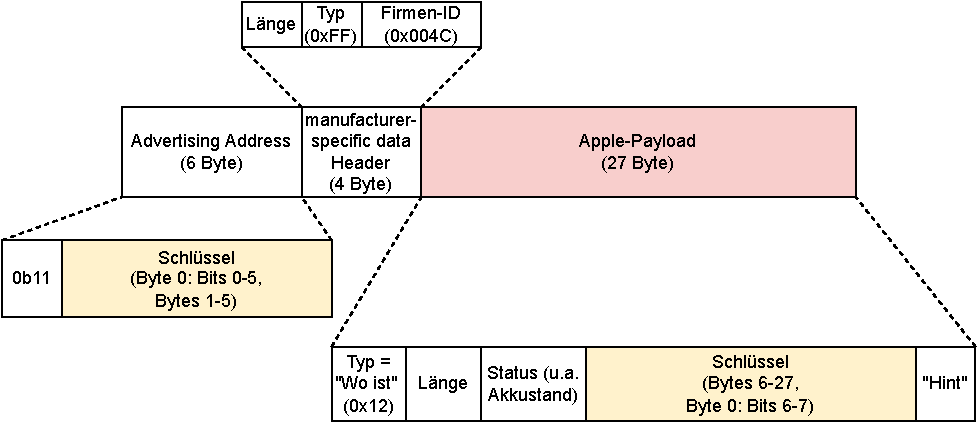
\includegraphics[width=0.9\textwidth]{apple_advertising.pdf}
    \caption{Aufbau der Advertisement Pakete des „Wo ist?“ Dienstes.}
    \label{fig:apple_advertising}
\end{figure}

Standardmäßig scannen alle Apple-Geräte (Finder-Devices) im Hintergrund nach Advertisements, die die Firmen-ID von Apple enthalten.
Wird ein Paket durch den Apple Payload Typ $0x12$ als Advertisement für den „Wo ist?“ Dienst identifiziert, wird vom Finder Device zunächst die aktuelle Position bestimmt und ein sogenannter \textit{Location Report} erstellt.
Das Format dieses Reports ist in \autoref{fig:location_report} gezeigt.
\begin{figure}
    \centering
    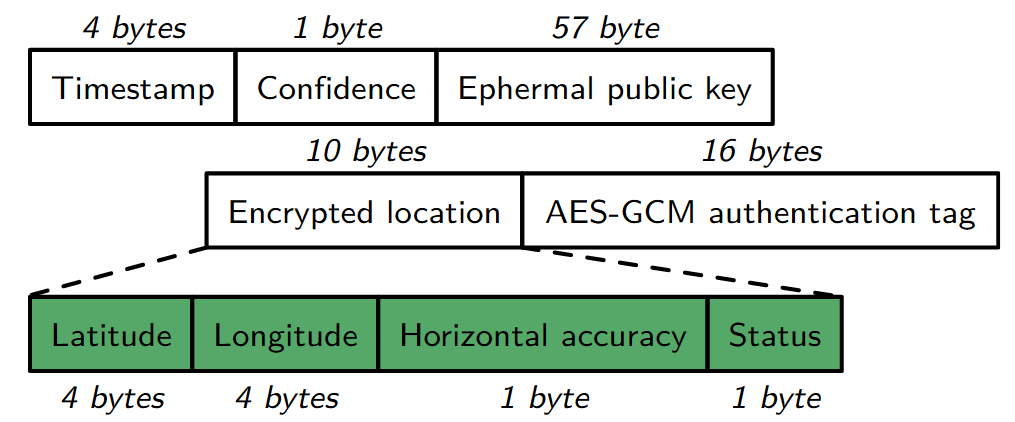
\includegraphics[width=0.85\textwidth]{location_report}
    \caption{Format des Location Reports \cite{Heinrich_FindMy}}
    \label{fig:location_report}
\end{figure}
Der Hauptbestandteil des Reports sind die wie oben beschrieben verschlüsselten Standortinformationen, bestehend aus Koordinaten, Genauigkeit und Status.
Außerdem sind sowohl der temporäre Schlüssel, welcher vom Finder-Device aus dem Advertisement Key abgeleitet und für den \ac{ECDH}-Schlüsselaustausch genutzt wurde, und der \ac{AES}-\ac{GCM} Authentication Tag teil des Reports.
Daneben findet sich unter anderem der Zeitstempel zum Zeitpunkt der Erstellung des Reports.
Beim Upload wird der Report mit einem \ac{SHA}-256 Hash des verwendeten Advertisement Keys verknüpft, um die Identifizierung zu ermöglichen \cite{Heinrich_FindMy}.
Im Vergleich zu konkurrierenden Diensten ist die Verschlüsselung ein wichtiger Schritt, um die Sicherheit und Privatsphäre des Dienstes zu verbessern.
Meist werden Reports nicht unmittelbar nach der Erstellung hochgeladen.
Stattdessen sammelt das Gerät mehrere Reports und lädt diese gebündelt hoch.
Der empfangende Server ordnet den Reports zusätzlich den Zeitstempel zum Zeitpunkt des Datenempfangs zu.
Tonetto \textit{et al.} \cite{Tonetto_FindMy} haben gezeigt, dass die Art der Internetverbindung beeinflusst, wann die Reports hochgeladen werden.
So liegt der Median für den Upload eines Reports bei aktiver WLAN-Verbindung bei 15 Minuten während bei aktiver Mobilfunkverbindung der Median bei 3 Stunden liegt.
Der Upload erfolgt über einen HTTPS-Request, der zusätzlich über den Header authentifiziert wird.
Dieser Header enthält unter anderem ein Identitäts-Zertifikat des Geräts und eine Signatur des Requests.
Diese Signatur wird mit dem privaten Schlüssel erstellt, welcher in einem speziellen Sicherheitsbereich, dem \textit{Secure Enclave Processor} des Geräts gespeichert ist, welcher das unberechtigte Auslesen verhindert.
Somit kann vermutlich sichergestellt werden, dass nur Apple Geräte in der Lage sind Reports hochzuladen, was das Erstellen gefälschter Reports erschwert \cite{Heinrich_FindMy}.


Um die Standortdaten vom Server abzurufen, wird ein über Basic Authentication mit der Apple-ID des Nutzers und einem Token authentifizierter, HTTPS-Request verwendet.
Die Anfrage enthält zusätzlich eine Liste der letzten Advertisement Keys des verlorenen Geräts.
So können die verschlüsselten Location Reports heruntergeladen und anschließend auf dem Gerät entschlüsselt werden, um das verlorene Gerät zu lokalisieren \cite{Heinrich_FindMy}.
\autoref{lst:findmy_result} zeigt die Struktur der Antwort auf einen solchen Request in gekürzter Form.
Die Antwort besteht aus einem Array von Objekten, die jeweils den Hash des Advertisement Keys, einen verschlüsselten Location Report und Metadaten, darunter den Zeitstempel des Datenempfangs, enthalten.
Anhand des Hashes kann der für die Entschlüsselung zu verwendende Advertising Key bestimmt werden.
Entschlüsselte Standortdaten aus mehreren Reports können kombiniert werden, um Genauigkeit bei der Positionsermittlung zu erhöhen.
Gleichzeitig können die Daten mehrerer Reports auch dazu verwendet werden, den Pfad des verlorenen Geräts zu rekonstruieren.
Dafür können bis zu sieben Tage alte Positionen vom Server abgerufen werden \cite{Heinrich_FindMy}.

\begin{lstlisting}[label=lst:findmy_result,caption={Beispielhafte Antwort beim herunterladen von Location Reports\cite{Heinrich_FindMy}.}]
{
    "results": 
    [
        {
            "datePublished": 1586804587284,
            "payload": "JETtmwIEzRBG ....",
            "description": "found",
            "id": "B6E5tpUPbuudAc ...",
            "statusCode": 0
        },
        ...
    ] ,
    "statusCode": "200"
}
\end{lstlisting}
\section{Missbrauch des „Wo ist?“ Dienstes}
\label{sec:Missbrauch}

Das Hauptangriffsziel für Angreifer des „Wo ist?“ Dienstes sind die Standortdaten der Nutzer.
Apple ergreift verschiedene Maßnahmen, um die Sicherheit der Standortdaten sicherzustellen, wie bei der Erläuterung der Funktionsweise in \autoref{sec:Funktionsweise_FindMy} bereits gezeigt wurde.
Untersuchungen, wie durch Tonetto \textit{et al.} \cite{Tonetto_FindMy} haben jedoch geyeigt, dass dennoch Missbrauchspotenzial besteh, gegen welches der Dienst nicht oder nicht ausreichend geschützt ist.
Zunächst werden in \autoref{tab:cia_findmy} die allgemeinen Sicherheitsziele Vertraulichkeit (\textit{Confidentiality}), Integrität (\textit{Integrity}) und Verfügbarkeit (\textit{Availability}) sowie mögliche Angriffsziele im Kontext des „Wo ist?“ Dienstes erklärt.
Darauf aufbauend wird gezeigt, wie die von Apple implementierten Sicherheitsmaßnahmen, viele Angriffsszenarien erfolgreich unterbinden können.
Im Anschluss werden in \autoref{sec:szenarien} konkrete Missbrauchsszenarien aufgezeigt werden, gegen welche Apple nur unzureichende Maßnahmen ergreift und welche somit die Sicherheit und Privatsphäre der Nutzer und sogar Dritter gefährden können.
Diese Szenarien werden in \autoref{sec:Gegenmassnahmen} wieder aufgegriffen und mögliche Gegenmaßnahmen durch Apple respektive die Nutzer vorgestellt.

\begin{table}[h]
  \caption{Sicherheitsziele des „Wo ist?“ Dienstes und mögliche Angriffsziele.}
  \label{tab:cia_findmy}
  \begin{tabularx}{\textwidth}{ |l|X|X| }
    \hline
    \textbf{Sicherheitsziel}  & \textbf{Beschreibung}                                               & \textbf{Angriffsziel}                                           \\
    \Xhline{0.5mm}
    \hline
    Vertraulichkeit           & Standortdaten sind nur befugten Personen zugänglich.                & Standort eines Nutzers oder eines Geräts erhalten.              \\
    \hline
    Integrität                & Standortdaten sind vor Manipulation geschützt.                      & Standortdaten eines Nutzers oder eines Geräts manipulieren.     \\
    \hline
    Verfügbarkeit             & Standortdaten können abgerufen werden.                              & Verhindern, dass Standortdaten abgerufen werden können.         \\
    \hline
  \end{tabularx}
\end{table}

Die von Heinrich \textit{et al.} \cite{Heinrich_FindMy} identifizierten Angreifermodelle in \autoref{fig:adversary_models} zeigen verschiedene Möglichkeiten, wie ein Angreifer versuchen kann, den Dienst anzugreifen.
Sie gehen von vier verschiedenen Angreifermodellen aus, die sich im Angriffsvektor unterscheiden.
Potenzielle Angriffe können demnach von lokal installierten Anwendungen, Geräten in \ac{BLE}-Reichweite, einem klassischen Netzwerkangreifer und dem Dienstanbieter, also von Apple ausgehen.
Für jeden Angriffsvektor werden verschiedene mögliche Ziele definiert.
\begin{figure}[ht]
  \centering
  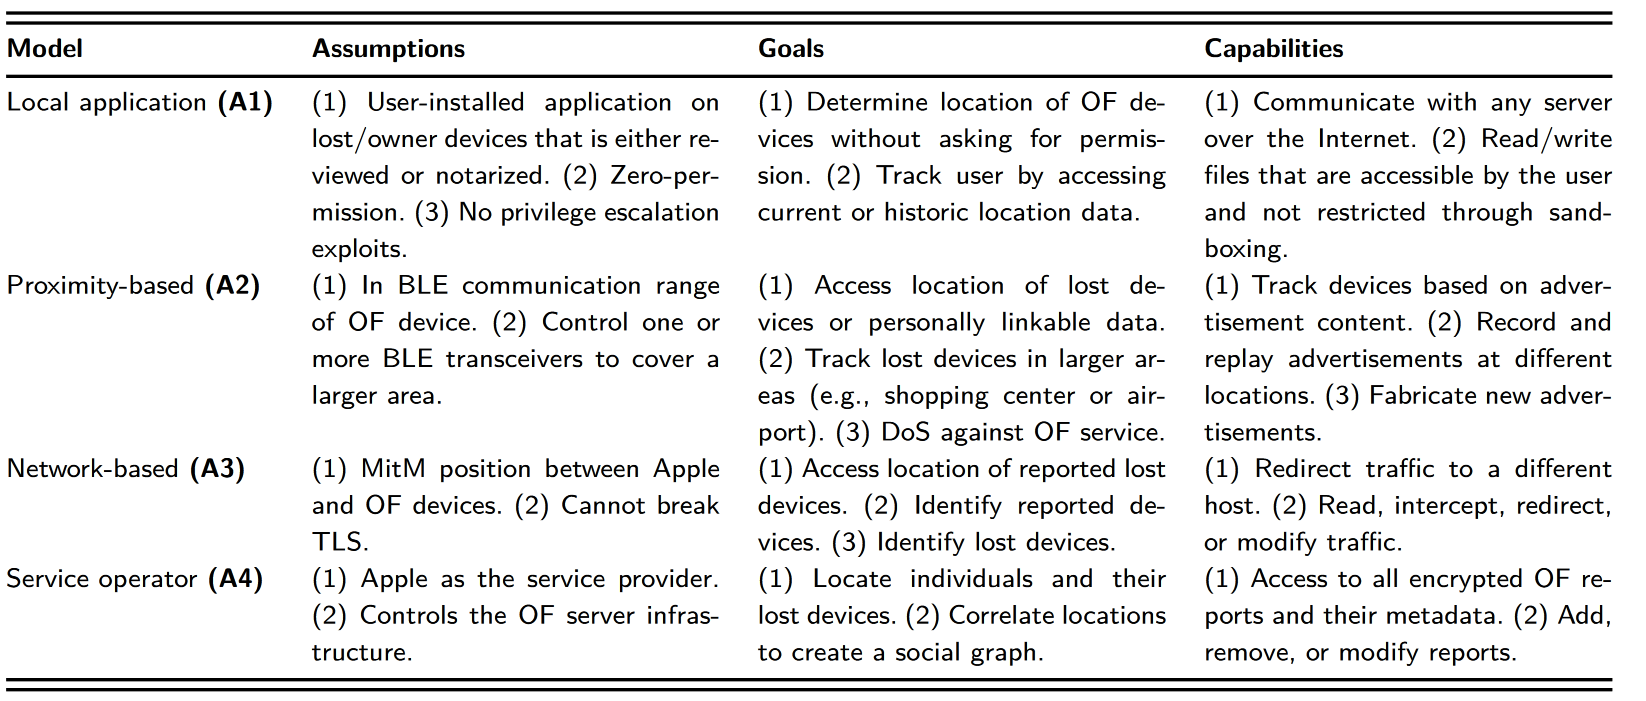
\includegraphics[width=\textwidth]{img/adversary_models}
  \caption{Angreifermodelle für den „Wo ist?“ Dienst \cite{Heinrich_FindMy}.}
  \label{fig:adversary_models}
\end{figure}

\autoref{tab:cia_adversary_models} ordnet den Zielen der einzelnen Angreifermodelle die betroffenen Sicherheitsziele zu.
\begin{table}[h]
  \caption{Zuordnung der Ziele der Angreifermodelle zu den allgemeinen Sicherheitszielen.}
  \label{tab:cia_adversary_models}
  \centering

  \begin{tabularx}{\textwidth}{ |l|X|X|l|X| }
    \hline
    \textbf{Angreifermodell}  & \textbf{Ziel} & \textbf{Vertraulichkeit} & \textbf{Integrität} & \textbf{Verfügbarkeit} \\
    \Xhline{0.5mm}
    \hline
    \multirow{2}{*}{A1} & (1) & \cmark & & \\
    \cline{2-5}
    & (2) & \cmark & & \\
    \hline
    \multirow{3}{*}{A2} & (1) & \cmark & & \\
    \cline{2-5}
    & (2) & \cmark & & \\
    \cline{2-5}
    & (3) & & & \cmark  \\
    \hline
    \multirow{3}{*}{A3} & (1) & \cmark & & \\
    \cline{2-5}
    & (2) & \cmark & & \\
    \cline{2-5}
    & (3) & \cmark & & \\
    \hline
    \multirow{2}{*}{A1} & (1) & \cmark & & \\
    \cline{2-5}
    & (2) & \cmark & & \\
    \hline
  \end{tabularx}
\end{table}
Dabei fällt auf, dass der Fokus auf der Vertraulichkeit der Daten liegt.
Sollten Angreifer Zugriff auf die Standortdaten erhalten, könnten sie diese für viele verschiedene Zwecke missbrauchen.
Zum Beispiel können diese Daten für gezielte Diskriminierung, Verfolgung und Überwachung durch Dritte oder auch durch staatliche Akteure verwendet werden.
Als personenbezogene Daten unterliegen die Standortdaten zusätzlich der \ac{DSGVO}.
Durch mögliche Rückschlüsse auf beispielsweise religiöse oder politische Überzeugungen sind Standortdaten nach Artikel 9 \ac{DSGVO} häufig auch als sensible personenbezogene Daten zu betrachten.
Deshalb ist Apple zumindest innerhalb der Europäischen Union auch verpflichtet, die Vertraulichkeit der Daten durch geeignete Maßnahmen zu schützen.
Wie bereits in \autoref{sec:Funktionsweise_FindMy} gezeigt, trifft Apple verschiedene Maßnahmen, die darauf abzielen die Vertraulichkeit zu wahren.
Die Auswirkungen dieser Maßnahmen werden in \autoref{sec:auswirkungen_sicherheitsmassnahmen} näher betrachtet.
Darüber hinaus werden in \autoref{sec:szenarien} mögliche Angriffe auf die Vertraulichkeit beschrieben, gegen welche die Sicherheitsmaßnahmen von Apple nicht ausreichend schützen.

Angriffe auf die Integrität und die Verfügbarkeit der Daten werden \cite{Heinrich_FindMy} nicht detailliert untersucht.
Nur das \textit{Proximity-based} Modell (A2 in \autoref{tab:cia_adversary_models}) zielt auch auf die Verfügbarkeit der Daten ab.
Wird die Verfügbarkeit beeinträchtigt, ist es für den Besitzer eines Geräts nicht mehr möglich, die aktuellen Standortdaten abzurufen.
Die Beeinträchtigung der Integrität der Daten wird nicht untersucht.
Jedoch ist ein gewisser Zusammenhang mit der Verfügbarkeit gegeben.
Durch gezielte Manipulation der Daten kann der Besitzer beispielsweise nicht mehr unterscheiden welche Daten korrekt sind, was die Verfügbarkeit stark beeinträchtigen kann.
Inwieweit Apples Sicherheitsmaßnahmen auch Integrität und Verfügbarkeit schützen, und welche Angriffe dennoch möglich sind, wird in \autoref{sec:auswirkungen_sicherheitsmassnahmen} und \autoref{sec:szenarien} näher betrachtet.


\subsection{Auswirkungen der Sicherheitsmaßnahmen}
\label{sec:auswirkungen_sicherheitsmassnahmen}

\subsubsection{Ende-zu-Ende Verschlüsselung}
Die Betrachtung der Funktionsweise in \autoref{sec:Funktionsweise_FindMy} zeigt, wie die Ende-zu-Ende-Verschlüsselung des Dienstes technisch umgesetzt wird.
Durch die Verwendung dieses Verschlüsselungsmechanismus kann unter der Annahme, dass der Angreifer die Verschlüsselung nicht brechen kann, gewährleistet werden, dass nur der Besitzer eines verlorenen Geräts die Standortdaten entschlüsseln kann.
Sollte einem Angreifer gelingen die Daten direkt von Apples Server abzurufen, oder über einen \ac{MITM} Angriff die verschlüsselten Daten zu erhalten, können diese ohne die nur auf den Owner Devices verfügbaren Schlüssel nicht entschlüsselt werden.
Dabei werden ein \ac{MITM}-Angriffe durch die Verwendung von \ac{TLS} mit Certificate Pinning bei der Kommunikation mit Apples Servern verhindert \cite{Heinrich_FindMy}.
Durch die Ende-zu-Ende Verschlüsselung werden alle vom Netzwerkangreifer (A3 in \autoref{fig:adversary_models}) ausgehenden Bedrohungen adressiert.
Die zur Entschlüsselung benötigten Schlüssel werden auf den Geräten des Besitzers in der als sicher geltenden iCloud Keychain gespeichert.
So werden auch die von lokalen Angreifern (A1 in \autoref{fig:adversary_models}) ausgehenden Bedrohungen behandelt.
Eine in \cite{Heinrich_FindMy} aufgedeckte Schwachstelle, die aufgrund von unsicherer Speicherung der Schlüssel unbefugten Zugriff auf die Standortdaten ermöglicht, wurde durch Apple mittlerweile behoben.
Zusätzlich wird es durch die Ende-zu-Ende-Verschlüsselung auch Apple unmöglich gemacht, auf die Standortdaten der Nutzer zuzugreifen, womit das Lokalisieren durch den Dienstanbieter (A4 mit Ziel (1) in \autoref{fig:adversary_models}) verhindert wird.
Außerdem verbessert die Verschlüsselung die Integrität der Daten, da einmal verschlüsselte Daten ohne Entschlüsselung nicht manipuliert werden können, ohne dass diese Manipulation erkannt werden kann.
Jedoch ist es möglich, dass die Standortdaten auf Basis eines Replay-Angriffes generiert wurden.
Auf dieses Szenario wird in \autoref{sec:szenarien} näher eingegangen.


\subsubsection{Schlüsselrotation}
Die Schlüsselrotation der Advertising Keys im Intervall von 15 Minuten bei Endgeräten und bis zu 24 Stunden bei Accesories, wie in \autoref{sec:Funktionsweise_FindMy} beschrieben, trägt ebenfalls zur Vertraulichkeit der Standortdaten bei.
Durch die regelmäßige Rotation der Schlüssel wird das Tracking von Geräten anhand der im Advertising gesendeten Daten erschwert.
Damit richtet sich diese Maßnahme gezielt gegen das Tracking durch einen Angreifer in der Nähe (A2 mit Ziel (2) in \autoref{fig:adversary_models}).
Außerdem müssten für einen solchen Angriff viele scannende Geräte so positioniert werden, dass auch bei Bewegung die Advertisement Pakete des zu verfolgenden Geräts von einem der Scanner erfasst wird.
Um größere Bereiche abzudecken, wären jedoch sehr viele scannende Geräte notwendig, was den Angriff bereits deutlich erschwert.
In Verbindung mit der Schlüsselrotation ist die Verfolgung, auch mit hohem Aufwand, nur für das Intervall der Schlüsselrotation möglich.
Allerdings können AirTags und Drittanbieterprodukte durch das längere Intervall für bis zu 24 Stunden über einen solchen Angriff verfolgt werden.
Für Angreifer ist der Angriff jedoch insgesamt so komplex, dass eine direkte Verfolgung des Opfers in den meisten Fällen praktikabler wäre.
Heinrich \textit{et al.} \cite{Heinrich_FindMy} betrachten die Schlüsselrotation als ausreichend, um die Verfolgung von Geräten nach diesem Muster zu verhindern.
Jedoch waren zum Zeitpunkt ihrer Analyse keine Geräte mit einem Intervall der Schlüsselrotation von mehr als 15 Minuten auf dem Markt.


\subsection{Missbrauchsszenarien ohne ausreichende Gegenmaßnahmen}
\label{sec:szenarien}

Im Folgenden sind sieben Missbrauchsszenarien aufgeführt, welche nicht ausreichend durch Gegenmaßnahmen unterbunden werden.
Gegen einige werden gar keine Maßnahmen getroffen, andere Gegenmaßnahmen lassen sich leicht umgehen und sind dementsprechend nicht ausreichend.
Weiterhin ist Szenario \nameref{missbrauch:4} nicht als negativer Missbrauch zu verstehen, da der „Wo ist?“ Dienst in diesem Fall nicht zur Beeinträchtigung, sondern zur Steigerung der Privatsphäre genutzt wird.
Weil dieser Anwendungsfall jedoch nicht von Apple vorgesehen ist, handelt es sich dennoch um Missbrauch.
Die Szenarien basieren größtenteils auf den Arbeiten von Heinrich \textit{et al.} \cite{Heinrich_FindMy}, Tonetto \textit{et al.} \cite{Tonetto_FindMy}, Mayberry \textit{et al.} \cite{Mayberry_Tracking} und Garg \textit{et al.} \cite{Garg_Secure_Tracker}.

\subsubsection[M1]{M1: Replay-Angriff}
\label{missbrauch:1}
Durch die Ende-zu-Ende-Verschlüsselung und den authentifizierten Upload der Standortdaten, kann die Integrität der Standortdaten in vielen Fällen geschützt werden.
Allerdings können über einen Replay-Angriff manipulierte Standortdaten, welche korrekt verschlüsselt sind und authentifiziert hochgeladen werden, auf Apples Server gelangen.
Somit kann die Integrität der abgerufenen Standortdaten nicht mehr gewährleistet werden.
Der Nutzer kann eventuell nicht mehr erkennen, welche Daten korrekt sind und kann somit keine verlässliche Standortinformation erhalten, was die Verfügbarkeit beeinträchtigt \cite{Heinrich_FindMy}.
Dieser Angriff entspricht dem \ac{DOS}-Angriff durch einen Angreifer in der Nähe (A2 mit Ziel (3) in \autoref{fig:adversary_models}).

Um einen solchen Angriff durchzuführen, kann ein Angreifer die Advertisement Pakete eines Gerätes aufzeichnen und an anderen Orten wieder abspielen.
Geräte in der Nähe empfangen diese Pakete und senden Standortdaten verschlüsselt und korrekt authentifiziert an Apple.
Der Besitzer erhält die manipulierten Standortdaten interpretiert diese als korrekt, oder kann nicht mehr erkennen, welche Daten korrekt sind.
Es ist unklar, ob Apple gegen diese Art der Manipulation Maßnahmen ergreift.


\subsubsection[M2.1]{M2.1: Angriff auf die Verfügbarkeit durch Angreifer mit physischem Zugriff}
\label{missbrauch:2.1}
Die Verfügbarkeit der Standortdaten ist für die Betrachtung im Rahmen dieser Arbeit weniger relevant, da das Design des Dienstes vergleichsweise wenige Auswirkungen auf die Verfügbarkeit hat.
Dennoch ist die Verfügbarkeit durch verschiedene Angriffe bedroht.
Zum Beispiel könnte ein direkter \ac{DOS} Angriff auf die Server von Apple erfolgen, was allerdings als unwahrscheinliches Bedrohungsszenario angesehen werden kann.
Relevanter ist ein Angriff durch einen Angreifer mit physischem Zugriff auf das Lost Device.
Beispielsweise in Zusammenhang mit Diebstahl eines Gegenstandes, an welchem ein AirTag befestigt ist, kann durch Zerstörung oder Entfernen der Batterie, verhindert werden, dass neue Standortinformationen hochgeladen werden.
In diesem Kontext ist auch das Entfernen des AirTags vom Gegenstand möglich um die weitere Lokalisierung zu verhindern.
Da keine neuen, gültigen Standortdaten erzeugt werden, ist die Verfügbarkeit eingeschränkt.

\subsubsection[M2.2]{M2.2: Angriff auf die Verfügbarkeit durch Angreifer in der Nähe}
\label{missbrauch:2.2}
Zur Einschränkung der Verfügbarkeit der Standortdaten, reicht es auch aus, wenn ein Angreifer sich in der Nähe des Geräts befindet.
Zum Beispiel ist bei dem von Garg \textit{et al.} \cite{Garg_Secure_Tracker} als sicher vorgeschlagenen Systemen neben dem Entfernen der Batterie auch das gezielte Entladen dieser ohne physischen Zugriff möglich.
Dieses System ist so gestaltet, dass der aktuelle Standort vom Finder Device an das Lost Device gesendet wird, welches die Daten verschlüsselt zurückgibt.
In diesem Szenario kann ein Angreifer durch häufiges senden von Standorten an das Lost Device unter Zuhilfenahme der energieintensiven Verschlüsselungsoperationen, die Batterie des Lost Devices entladen.
Ein Angriff nach diesem Schema kann auch Apples System betreffen.
Insbesondere für Accessories geringer Batteriekapazität ist die gezielte Entladung ein relevantes Bedrohungsszenario.
Da jedoch beim „Wo ist?“ Dienst die Verschlüsselung nicht auf dem Lost Device erfolgt, muss der Angriff leicht variiert werden.
Accessories müssen die Möglichkeit bieten, einen Ton abzuspielen \cite{Apple_FindMySpec}.
Diese Funktion kann durch jeden in \ac{BLE}-Reichweite ausgelöst werden \cite{Heinrich_AirGuard} und genutzt werden, um die Batterie zu entladen.

\subsubsection[M3]{M3: Direktes Tracking von Personen}
\label{missbrauch:3}
Das Szenario des direkten Tracking von Personen bezieht sich auf die Verfolgung durch AirTags oder andere kleine Tracker.
Durch die kleine Größe der Tracker können diese in Jacken, Rucksäcken oder an Fahrzeugen befestigt werden, um einzelne Personen gezielt zu verfolgen.
Dieser Angriff wurde bereits vielfach in der Praxis beobachtet und für Stalking oder Autodiebstahl genutzt \cite{NYT_Airtags}.
Der „Wo ist?“ Dienst bietet zwar eine Funktion zur „Unwanted tracking detection“, um Nutzer auf mögliche Verfolgung hinzuweisen \cite{Apple_FindMySpec}.
Allerdings wurde bereits gezeigt, dass diese Funktion leicht umgangen werden kann \cite{Mayberry_Tracking} und in vielen Fällen nicht zuverlässig vor Tracking warnen kann \cite{Heinrich_AirGuard}.
Darüber hinaus ist die Funktion nur für iOS-Geräte direkt verfügbar, sodass für Android-Nutzer keinerlei Warnung erfolgt.
Demnach sind die Gegenmaßnahmen des „Wo ist?“ Dienstes gegen das direkte Tracking von Personen nicht als ausreichend zu bewerten.


\subsubsection[M4]{M4: Indirektes Tracking von Personen}
\label{missbrauch:4}
Beim indirekten Tracking werden Personen nicht durch Tracker direkt verfolgt.
Stattdessen werden anhand der Uploadzeitpunkte von Location Reports Rückschlüsse auf die Bewegung von Personen gezogen.
Dieses Missbrauchsszenario wurde von Tonetto \textit{et al.} \cite{Tonetto_FindMy} vorgestellt und kann nicht nur für das schadhafte Tracking von Personen genutzt werden, sondern auch als privatsphärefreundliche Funktion zum Crowd-Monitoring.
Da Finder Devices Location Reports generell gebündelt hochladen, und Apples Server die Uploadzeitpunkte mit einer Genauigkeit von wenigen Millisekunden speichern, ist es für Angreifer möglich, Location Reports, die vom gleichen Gerät stammen, anhand der Uploadzeitpunkte zu identifizieren \cite{Tonetto_FindMy}.
Während Finder Devices mit Mobilfunkverbindung Location Reports in der Regel erst nach einigen Stunden hochladen, erfolgt der Upload bei einer WLAN-Verbindung deutlich schneller.
Wechselt ein Finder Device von einer Mobilfunkverbindung zu einer WLAN-Verbindung, werden die zwischengespeicherten Location Reports in der Regel kurz darauf hochgeladen.
Unter der Annahme, dass Personen außerhalb einiger weniger Orte, wie zum Beispiel der eigenen Wohnung, nicht dauerhaft mit einem WLAN-Netzwerk verbunden sind, werden außerhalb dieser Orte erstellte Location Reports in etwa zur gleichen Zeit hochgeladen \cite{Tonetto_FindMy}.

Platziert ein Angreifer mehrere Tracker an verschiedenen Orten, erfassen Finder Devices diese und generieren jeweils Location Reports.
Jeder dieser Location Reports gibt an, zu welchem Zeitpunkt das Finder Device an welcher Position war.
Werden diese Location Reports gebündelt hochgeladen, kann der Angreifer die zusammengehörigen Location Reports anhand der Uploadzeitpunkte identifizieren.
Aus den Positionen und Zeitpunkten der Erstellung der Reports kann die Bewegung des Finder Device rekonstruiert werden \cite{Tonetto_FindMy}.


Zum privatsphärefreundlichen Crowd-Monitoring werden einzelne Tracker an öffentlichen Orten platziert.
Finder Devices, die sich in der Nähe dieser Tracker befinden, generieren Location Reports.
Diese Reports können von Apples Servern heruntergeladen werden und erlauben über die Anzahl der Reports Rückschlüsse auf die Anzahl der Personen, die sich in der Nähe des Trackers aufgehalten haben.
Über die Verwendung mehrere Tracker lassen sich auch die Bewegungen von Menschenmassen rekonstruieren.
Dieser Missbrauch des „Wo ist?“ Dienstes kann als Alternative zu aktuellen Bilderkennungs-basierten Crowd-Monitoring-Systemen verwendet werden und erlaubt eine ähnliche Genauigkeit.
Zusätzlich ist dieser Ansatz besser für die Privatsphäre der Betroffenen als die Bilderkennung, da keine personenbezogenen Daten erhoben werden \cite{Tonetto_FindMy}.


\subsection{M5: Verdeckter Datentransfer}
\label{missbrauch:5}
Tonetto \textit{et al.} \cite{Tonetto_FindMy} und Bräunlein \cite{braeunlein_sendmy} zeigen unabhängig voneinander, dass der „Wo ist?“ Dienst auch für einen verdeckten Datentransfer mit einer niedrigen Übertragungsrate ausgenutzt werden kann.
Dabei werden Finder Devices dazu genutzt, Daten an Apples Server zu übertragen, welche vom Angreifer heruntergeladen und dekodiert werden können.
Beide verwenden für das Senden der Daten einen Nachbau eines AirTags, bestehend aus einem \ac{BLE}-fähigen Mikrocontroller.

Bräunlein \cite{braeunlein_sendmy} kodiert eine zu sendende Nachricht in den im Advertisement gesendeten Daten.
Für jedes Bit der Nachricht wird ein 28 Byte langes Array, bestehend aus der Position des Bits in der Nachricht, einer ID des Senders und dem Wert des Bits generiert.
Anstatt einen öffentlichen Schlüssel im Advertisement zu senden, werden die so kodierten Daten für eine definierte Zeitspanne gesendet.
Danach wird der Prozess für das nächste Bit der Nachricht wiederholt.
Diese Kodierung ist in \autoref{fig:sendmy_encoding} schematisch dargestellt.
\begin{figure}[ht]
  \centering
  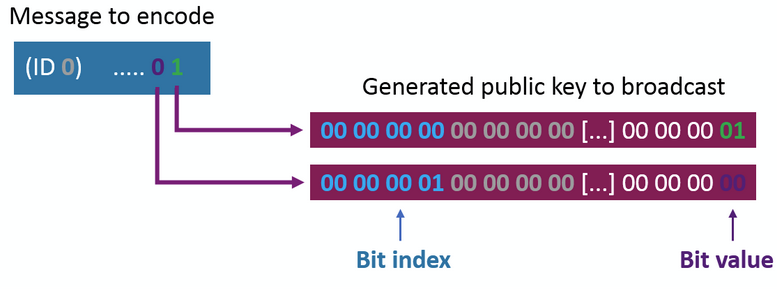
\includegraphics[width=0.9\linewidth]{sendmy_encoding.png}
  \caption{Bitweise Kodierung der Nachricht in im Advertisement übertragenen Daten \cite{braeunlein_sendmy}.}
  \label{fig:sendmy_encoding}
\end{figure}
Der Empfänger kann für jedes Bit der Nachricht die zwei möglichen Arrays generieren und eine Anfrage mit den jeweiligen \ac{SHA}-256 Hashes an Apples Server senden.
Abhängig davon, welcher der beiden Hashes in der Antwort enthalten ist, kann der Empfänger das Bit der Nachricht bestimmen.
Dabei wird ausgenutzt, dass jedes Apple Gerät die verschlüsselten Location Reports für beliebige öffentliche Schlüssel herunterladen kann.
Da die Location Reports Ende-zu-Ende verschlüsselt sind, wird dadurch die Vertraulichkeit nicht gefährdet.
Jedoch ist für dieses Missbrauchszenario die Entschlüsselung der Daten nicht notwendig, da lediglich das Vorhandensein eines bestimmten Location Reports überprüft werden muss, um die Nachricht zu dekodieren.
Ein Nachteil bei diesem Verfahren ist, dass somit auch jedes Apple-Gerät die Nachricht abrufen könnte.


Das von Tonetto \textit{et al.} \cite{Tonetto_FindMy} vorgestellte Verfahren verwendet 16 bekannten Advertising Keys, um die Nachricht in eine Folge dieser Keys zu kodieren.
Dazu wird eine Menge von Advertising Keys zuvor generiert und zwischen Sender und Empfänger ausgetauscht.
Der Sender kann die Nachricht erzeugt aus der Nachricht eine Abfolge der Advertising Keys und sendet diese nacheinander im Advertisement.
Finder Devices, die sich in der Nähe befinden, empfangen die Advertisements, erstellen Location Reports und laden diese hoch.
Der Empfänger der Nachricht kann alle Location Reports der bekannten Advertising Keys herunterladen, die Daten entschlüsseln und anhand der Zeitstempel die Folge und damit die ursprüngliche Nachricht rekonstruieren.
Im Vergleich zum Verfahren von Bräunlein, werden hier echte Advertising Keys verwendet, sodass die Location Reports entschlüsselt werden können, sodass der Standort des Senders bestimmt werden kann.
Zusätzlich muss der Empfänger weniger Anfragen an Apples Server stellen, da nur 16 unterschiedliche Advertising Keys verwendet werden.
Bräunleins Verfahren benötigt zwei Anfragen an Apples Server pro übertragenem Bit.


\subsection{M6: Korrelation von Standorten durch Apple}
\label{missbrauch:6}

Das zweite Ziel des Angreifermodells des Dienstanbieters (A4 in \autoref{fig:adversary_models}) bezieht sich auf die Korrelation von Standorten mehrerer Nutzer.
Heinrich \textit{et al.} \cite{Heinrich_FindMy} zeigen, dass durch den authentifizierten Up- und Download, die Korrelation durch Apple theoretisch möglich ist.
Die konkreten Standorte können aufgrund der Ende-zu-Ende-Verschlüsselung nicht bestimmt werden.
Allerdings kann bestimmt werden, welches Gerät welche Location Reports erstellt und welcher Nutzer diese heruntergeladen hat.
Daraus lässt sich folgern, welche Nutzer sich zu welcher Zeit an einem gemeinsamen Ort aufgehalten haben.
Apple könnte diese Informationen nutzen, um soziale Beziehungen zwischen Nutzern zu bestimmen und diese, zum Beispiel zu Werbezwecken, zu analysieren.
In \cite{Heinrich_FindMy} wird zusätzlich aufgezeigt, dass diese Daten auch von Strafverfolgungsbehörden genutzt werden könnten, um unter anderem die Identität von Demonstrationsteilnehmern zu bestimmen.
Jedoch ist nicht klar, ob Apple diese Daten tatsächlich speichert und nutzt.

\section{Konkrete Missbrauchsszenarien ohne ausreichende Gegenmaßnahmen}
\label{sec:szenarien}

Basierend auf den Arbeiten von Heinrich \textit{et al.} \cite{Heinrich_FindMy}, Tonetto \textit{et al.} \cite{Tonetto_FindMy}, Mayberry \textit{et al.} \cite{Mayberry_Tracking} und Garg \textit{et al.} \cite{Garg_Secure_Tracker}, sind im Folgenden sechs Missbrauchsszenarien aufgeführt, welche nicht ausreichend durch Gegenmaßnahmen unterbunden werden.
Gegen einige werden gar keine Maßnahmen getroffen, andere Gegenmaßnahmen lassen sich leicht umgehen und sind dementsprechend nicht ausreichend.
Neben der Erläuterung des Szenarios werden jeweils Gegenmaßnahmen vorgeschlagen, welche von Apple oder den Nutzern des Dienstes beziehungsweise den Betroffenen umgesetzt werden können.
In diesem Zusammenhang werden auch mögliche Problem dieser Gegenmaßnahmen aufgezeigt.

Weiterhin ist Szenario \nameref{missbrauch:4} differenziert zu betrachten, da es sowohl einen negativen als auch einen positiven Missbrauch des Dienstes beschreibt.
Im einen Fall lässt sich der Dienst missbrauchen, um die Privatsphäre Dritter einzuschränken.
Im anderen Fall erfolgt der Missbrauch, zum besseren Schutz der Privatsphäre.
Weil dieser Anwendungsfall jedoch nicht von Apple vorgesehen ist, handelt es sich dennoch um Missbrauch.


Allgemein konnten keine Gegenmaßnahmen identifiziert werden, welche jedes der Szenarien unterbinden können.
Die Nutzer des „Wo ist?“ Dienstes können sich jedoch gegen alle Missbrauchsszenarien außer \nameref{missbrauch:3} schützen, indem sie den Dienst nicht nutzen und der Teilnahme als Finder Devices widersprechen.
Diese Gegenmaßnahme wird allerdings nicht als sinnvoll angesehen, da der Dienst potenziell sehr nützlich sein kann.
Stattdessen werden, wenn möglich, zu den jeweiligen Szenarien Gegenmaßnahmen vorgestellt, die eine möglichst uneingeschränkte Nutzung des Dienstes erlauben.

%TODO: 
Dennoch gibt es eine Gegenmaßnahme, welche \nameref{missbrauch:5} sicher verhindert und das Umgehen der bestehenden Maßnahmen gegen \nameref{missbrauch:3} verhindert.
Dazu muss der Einsatz inoffizieller Tracker verhindert werden.
Zur sicheren Verhinderung des Einsatzes von inoffiziellen Trackern müsste Apple beispielsweise eine Authentifizierung für alle Tracker umsetzen, was laut Mayberry \textit{et al.} \cite{Mayberry_Tracking} nicht ohne erhebliche Anpassungen der offiziellen Tracker möglich ist.
Eine weitere Möglichkeit wäre die Registrierung aller offiziellen Tracker mitsamt \ac{MBK}, um erkennen zu können, ob ein Location Report mit einem gültigen Schlüssel erzeugt wurde.
Da diese Methode jedoch die Ende-zu-Ende-Verschlüsselung der Location Reports aufweicht, sodass Apple die Daten entschlüsseln kann, wird sie als nicht geeignet angesehen.



\subsection[M1]{M1: Replay-Angriff}
\label{missbrauch:1}
Durch die Ende-zu-Ende-Verschlüsselung und den authentifizierten Upload der Standortdaten, kann die Integrität der Standortdaten in vielen Fällen geschützt werden.
Allerdings können Replay-Angriffe genutzt werden, um dafür zu sorgen, dass manipulierte Standortdaten auf Apples Server und auf das Owner Device gelangen.
Diese sind korrekt verschlüsselt und werden ebenfalls korrekt authentifiziert hochgeladen, sodass für Apples Server keine triviale Möglichkeit besteht die Manipulation zu erkennen.

Durch Replay-Angriffe kann die Integrität der abgerufenen Standortdaten nicht mehr gewährleistet werden.
Der Nutzer kann bei abgerufenen widersprüchlichen Standortinformationen nicht zwischen korrekten und manipulierten Daten unterscheiden und erhält somit keine verlässlichen Standortinformationen, was die Verfügbarkeit beeinträchtigt \cite{Heinrich_FindMy}.
Dieser Angriff entspricht im wesentlichen \ac{DOS}-Angriff durch einen Angreifer in der Nähe (A2 mit Ziel (3) in \autoref{fig:adversary_models}).
Allerdings kann hier das Ziel auch in der reinen Manipulation der Standortdaten liegen, die Verfügbarkeit muss nicht in jedem Fall betroffen sein.
\begin{figure}[ht]
    \centering
    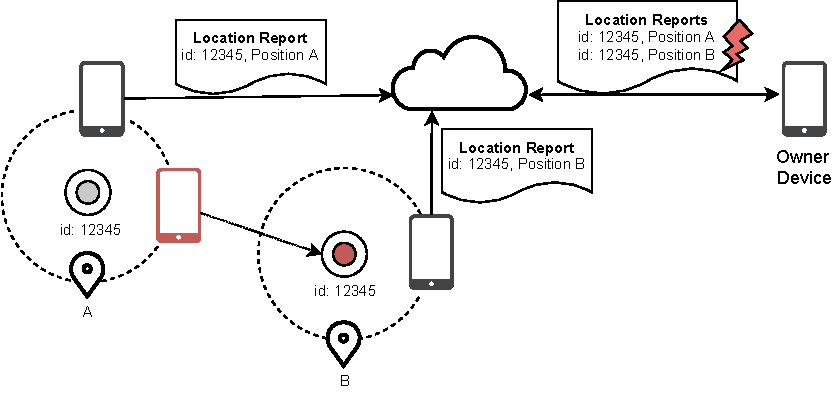
\includegraphics[width=0.9\textwidth]{replay.pdf}
    \caption{Schema eines Replay-Angriffs um die Integrität verfügbarer Standortdaten zu beeinträchtigen.}
    \label{fig:replay_attack}  
\end{figure}

Das grundsätzliche Schema eines Replay-Angriffs ist in \autoref{fig:replay_attack} dargestellt.
Um einen solchen Angriff durchzuführen, zeichnet ein Angreifer zunächst die Advertisement-Pakete und damit den öffentlichen Advertising Key eines Lost Device auf.
Anschließend kann der Angreifer die Aufzeichnung zu einer anderen Zeit oder an einem anderen Ort senden.
Geräte in der Nähe empfangen die wiederholten Pakete und erstellen Location Reports, welche mit dem enthaltenen Advertising Key verschlüsselt werden.
Bei einer Anfrage erhält das Owner Device beispielsweise sowohl korrekte als auch manipulierte Standortdaten.
Das Owner Device kann nicht bestimmen, welche Informationen korrekt sind und die Daten daher nicht für die Lokalisierung des Lost Device verwenden.

\subsubsection{Gegenmaßnahmen}
Das Design des Dienstes lässt es prinzipiell zu, Replay-Angriffe zumindest zu erkennen.
Die „Wo ist?“ App könnte beispielsweise die Plausibilität der empfangenen Standortdaten prüfen und Nutzer auf eventuelle Manipulationen hinweisen.
Eine solche Prüfung wäre unter anderem anhand der Zeitpunkte der Standortdaten möglich.
Große Abweichungen des Standorts bei Reports, welche kurz nacheinander oder gleichzeitig erstellt wurden, könnten als nicht realistisch erkannt werden.
Allerdings lassen sich so nicht alle Manipulationen erkennen, da der Replay-Angriff zum Beispiel auch in der Nähe des tatsächlichen Standorts durchgeführt werden kann, sodass die Abweichungen der Standorte klein sind.
In diesem Fall wird lediglich die Genauigkeit der Lokalisierung eingeschränkt.
Außerdem könnte das Owner Device bestimmen, welcher Advertising Key zum Zeitpunkt der Generierung des Location Reports aktiv war und so überprüfen ob der Location Report mit dem passenden Advertising Key erstellt wurde, oder ob ein älterer Schlüssel verwendet wurde.
So lassen sich mögliche Replay-Angriffe auf das Intervall der Schlüsselrotation beschränken.

Jedoch sind diese Maßnahmen nur durch Apple, durch eine Aktualisierung der „Wo ist?“ App umsetzbar. 
Auf Apples Server können Manipulationen hingegen nicht erkannt werden, da durch die Verschlüsselung kein Zugriff auf die Standortinformationen besteht.

Die Nutzer haben keine Möglichkeit, sich vor einem Replay-Angriff zu schützen.
Sobald ein Gerät Advertisement-Pakete sendet, könnten diese von einem Angreifer aufgezeichnet und für einen Replay-Angriff verwendet werden.


\subsection[M2]{M2: \ac{DOS}: Angreifer in der Nähe}
\label{missbrauch:2}
Die Verfügbarkeit der Standortdaten ist für die Betrachtung im Rahmen dieser Arbeit weniger relevant, da das Design des Dienstes vergleichsweise wenige Auswirkungen auf die Verfügbarkeit hat.
Dennoch ist die Verfügbarkeit durch verschiedene Angriffe bedroht.
Die Verfügbarkeit von Standortdaten lässt sich durch den Missbrauch von Funktionen des Dienstes durch einen Angreifer in \ac{BLE}-Reichweite eines Lost Device beeinträchtigen.
Dieser Angriff entspricht dem dritten Ziel des Angreifers in der Nähe (A3 mit Ziel (3) in \autoref{fig:adversary_models}).

Garg \textit{et al.} \cite{Garg_Secure_Tracker} zeigen bei einem von ihnen entwickelten Crowdsourced-Tracking Dienst, dass ein Angreifer in der \ac{BLE}-Reichweite des Geräts in der Lage ist, die Batterie des Geräts gezielt zu entladen.
Beim betroffenen System wird der aktuelle Standort vom Finder Device an das Lost Device gesendet, welches die Daten verschlüsselt zurückgibt.
Da sowohl Verschlüsselung als auch aktive \ac{BLE}-Kommunikation vergleichsweise energieintensiv sind, kann ein Angreifer durch das häufige Anfragen der Verschlüsselung die Batterie des Gerät entladen.

Ein Angriff nach diesem Schema kann prinzipiell auch Apples System betreffen.
Insbesondere für Accessories mit üblicherweise geringer Batteriekapazität ist die gezielte Entladung ein relevantes Bedrohungsszenario.
Da jedoch beim „Wo ist?“ Dienst die Verschlüsselung nicht auf dem Lost Device erfolgt, muss der Angriff leicht variiert werden.
Laut Apples Spezifikation müssen Accessories die Möglichkeit bieten, einen Ton abzuspielen.
Diese Funktion ist Teil der \ac{UT} und soll Nutzer vor direktem Tracking, wie in \nameref{missbrauch:3} beschrieben, warnen und das Auffinden versteckter Tracker ermöglichen \cite{Apple_FindMySpec}.
Allerdings kann diese Funktion durch alle Geräte in \ac{BLE}-Reichweite missbraucht werden, um Töne abzuspielen \cite{Heinrich_AirGuard}.
Das Abspielen von Tönen ließe sich im Rahmen eines Angriffes so lange wiederholen, bis die Batterie des Lost Devices entladen ist.

\subsubsection{Gegenmaßnahmen}
Schutz gegen die Entladung der Batterie durch Angreifer in der Nähe ist nur schwierig umsetzbar.
Da bei Apples System die Verschlüsselung nicht auf dem verlorenen Gerät, sondern auf dem Finder Device erfolgt, ist dieser Angriff vermutlich aufwändiger als beim System von Garg \textit{et al.} \cite{Garg_Secure_Tracker}.
Außerdem ist das Abspielen eines Tons vergleichsweise auffällig und damit für Angreifer nicht in jeder Situation gut geeignet.

Als Gegenmaßnahme könnte Apple die Funktion Töne abzuspielen entfernen, was den Angriff nicht komplett verhindern, aber erschweren kann.
Allerdings ist diese Funktion Teil der Schutzmaßnahmen gegen direktes Tracking und die Entfernung dieser Funktion würde die Maßnahmen zur \ac{UT} abschwächen.

Die Nutzer haben kaum Möglichkeiten sich gegen dieses Szenario zu schützen. 
Das Entfernen des Lautsprechers von Accessories wäre eine Möglichkeit die Entladung durch Angreifer in der Nähe zu erschweren.
Da die Entladung durch das Abspielen von Tönen jedoch auffällig und demnach als eher unwahrscheinlich anzusehen ist, ist diese Maßnahme nur bedingt sinnvoll.


\subsection[M3]{M3: Direktes Tracking von Personen}
\label{missbrauch:3}
Das Szenario des direkten Trackings von Personen bezieht sich auf die Verfolgung durch AirTags oder andere kleine Tracker.
Durch die kleine Größe der Tracker können diese in Jacken, Rucksäcken oder an Fahrzeugen befestigt werden, um einzelne Personen gezielt zu verfolgen \cite{Roth_airtags}.
Finder Devices in der Nähe der Tracker erzeugen Location Reports, die ein Angreifer zur Bestimmung der Position der Tracker und damit der Position des Opfers abrufen kann.
Solche Angriffe wurden bereits vielfach in der Praxis beobachtet und für Stalking oder Autodiebstahl genutzt \cite{NYT_Airtags}.
Dieses Szenario lässt sich keinem der Angreifermodelle von Heinrich \textit{et al.} \cite{Heinrich_FindMy} zuordnen, da es keinen Angriff auf den Dienst, sondern ein gezielter Missbrauch des Dienstes darstellt.
Der Angreifer ist ein legitimer Nutzer des Dienstes, der ein Lost Device lokalisiert.
Lediglich die Platzierung des Lost Devices unterscheidet diesen Angriff von einem normalen Einsatz des Dienstes.

Der „Wo ist?“ Dienst bietet zwar eine Funktion, um Nutzer auf mögliche Verfolgung hinzuweisen (\ac{UT}) \cite{Apple_FindMySpec}.
Diese ist nur für iOS automatisch verfügbar, sodass Android-Nutzer ohne eigenes Zutun nicht geschützt werden können.
Zusätzlich lässt sich die Funktion durch den Einsatz inoffizieller Tracker leicht umgehen und kann in vielen Fällen nicht zuverlässig vor Tracking warnen \cite{Heinrich_AirGuard,Mayberry_Tracking}.
Inoffiziell sind alle Tracker, welche den „Wo ist?“ Dienst ohne explizite Erlaubnis von Apple nutzen.
Solche Tracker lassen sich leicht aus kostengünstiger \ac{BLE}-Hardware und Open-Source-Software zusammenbauen und sind häufig günstiger als offizielle AirTags \cite{Heinrich_OpenHaystack,Mayberry_Tracking}.
Kennzeichen dieser Tracker ist die Möglichkeit, im Advertisement beliebige Daten zu senden, was genutzt werden kann, um die \ac{UT} zu umgehen \cite{Mayberry_Tracking}.

Da die Gegenmaßnahmen des „Wo ist?“ Dienstes gegen das direkte Tracking von Personen einfach umgangen werden können, sind sie als nicht ausreichend zu bewerten.

\subsubsection{Gegenmaßnahmen}

Die aktuell von Apple umgesetzte \ac{UT} setzt sich aus verschiedenen Funktionen zusammen.
Teile davon müssen von den Accessories implementiert werden, andere sind in iOS integriert.

Accessories müssen zum Beispiel einen Ton abspielen, wenn sie mindestens drei Tage vom Gerät des Besitzers getrennt sind und Bewegung erkennen \cite{Apple_FindMySpec}.
Da der Lautsprecher bei AirTags beispielsweise einfach entfernt werden kann, und AirTags ohne Lautsprecher auf verschiedenen Online-Marktplätzen erhältlich sind, trägt diese Funktion kaum zum Schutz vor Stalking bei \cite{Heinrich_AirGuard}.
Zusätzlich zeigen Roth \textit{et al.} \cite{Roth_airtags}, dass die Firmware von AirTags manipuliert werden kann, um diese Funktion zu deaktivieren oder anzupassen.

Weiterhin kann iOS die Verfolgung durch ein Accessory eines anderen Nutzers erkennen und eine Warnung anzeigen.
Diese Funktion beruht darauf, dass Accessories im Separated State ihren Advertising Key nur alle 24 Stunden wechseln.
So lassen sich Accessories anhand der \ac{BLE}-Advertisements über länger Zeiträume erkennen.
Wird ein Accessory seit mehr als zehn Minuten in der Nähe erkannt und ist es dem Gerät mindestens 840 Meter gefolgt, wird es als verdächtig markiert \cite{Heinrich_AirGuard}.
Warnungen werden allerdings, zur Vermeidung von false positives, verzögert angezeigt.
Heinrich \textit{et al.} \cite{Heinrich_AirGuard} zeigen, dass die Warnungen erst mehrere Stunden nach der Erkennung oder bei Rückkehr des Benutzers an den von iOS als Zuhause bestimmten Ort angezeigt werden.
Ein Angreifer kann die Position seines Opfers also, ohne die \ac{UT} umgehen zu müssen, mindestens mehrere Stunden oder sogar bis zu dessen Zuhause verfolgen, ohne eine Warnung auszulösen.
Besitzt das Opfer kein Apple-Gerät, ist eine unbegrenzte Verfolgung möglich.

Inzwischen bietet Apple auch eine App für Android an, um die Warnung vor Tracking auch für Android-Nutzer zu ermöglichen, welche jedoch von Heinrich \textit{et al.} \cite{Heinrich_AirGuard} mangels Features nicht als ausreichend angesehen wird.
Die Open-Source App \textit{AirGuard} für Android bietet eine ähnliche Warnfunktion, welche in Tests besser abschneidet als die Warnfunktion von iOS und die offizielle App von Apple.
Für iOS ist dieser bessere Schutz aufgrund von Einschränkungen der Bluetooth-\acp{API} für Apps von Drittanbietern nicht verfügbar \cite{Heinrich_AirGuard}.

Problematisch ist ebenfalls, dass die \ac{UT} von iOS durch den Einsatz inoffizieller Tracker einfach und zuverlässig umgangen werden kann \cite{Heinrich_AirGuard,Mayberry_Tracking}.
Einerseits können inoffizielle Tracker für Status-Feld im Advertisement-Format von Apple immer den Wert 0 senden, was den Tracker als verlorenes Endgerät ausweist.
Verlorene Endgeräte werden für das \ac{UT}-Feature nicht betrachtet und generieren deshalb keine Warnungen \cite{Heinrich_AirGuard,Mayberry_Tracking}.
Die AirGuard-App hingegen warnt unabhängig vom Status-Feld \cite{Heinrich_AirGuard}, was zeigt, dass zumindest diese Möglichkeit zur Umgehung einfach behoben werden kann.

Andererseits können Tracker den Advertising Key häufig wechseln, sodass iOS nicht erkennen kann, ob es sich um den gleichen Tracker handelt.
Damit ist keine Unterscheidung von Trackern und Endgeräten ohne Internetverbindung und keine Warnungen mehr möglich \cite{Mayberry_Tracking}.
Würde auch vor Endgeräten ohne Internetverbindung gewarnt, würden vermutlich sehr viele falsche Warnungen generiert werden.
Die einzige sichere Möglichkeit, ist die Verwendung inoffizieller Tracker zu verhindern, wie oben bereits beschrieben.


Nutzer können sich vor Tracking durch offizielle Tracker warnen lassen, indem sie entweder ein iOS-Gerät, oder die AirGuard-App verwenden.
Weiterhin können inoffizielle Tracker, welche nur das Status-Feld manipulieren, von der AirGuard-App erkannt werden und Android-Nutzer können auch in diesem Fall gewarnt werden.
Durch manuelle \ac{BLE}-Scans der Umgebung haben Nutzer von AirGuard außerdem die Möglichkeit, beliebige „Wo ist?“-Geräte in der Nähe zu erkennen.
Durch die beschriebenen Einschränkungen müssen Nutzer jedoch selbst Entscheiden, ob ein Gerät als schadhafter Tracker einzustufen ist.



\subsection[M4]{M4: Indirektes Tracking von Personen}
\label{missbrauch:4}
Beim indirekten Tracking werden Personen nicht durch versteckte Tracker direkt verfolgt.
Stattdessen werden anhand der Uploadzeitpunkte von Location Reports Rückschlüsse auf die Bewegung von Personen gezogen.
Dieses Missbrauchsszenario wird von Tonetto \textit{et al.} in \cite{Tonetto_FindMy} vorgestellt und kann nicht nur für das schadhafte Tracking von Personen genutzt werden.
Stattdessen kann es auch zu Zwecken des Crowd-Monitorings genutzt werden und stellt dabei einen kleineren Eingriff in die Privatsphäre betroffener dar als alternative Methoden. 

Der Missbrauch beruht darauf, dass Location Reports generell gebündelt hochgeladen, und Apples Server den jeweiligen Uploadzeitpunkt mit einer Genauigkeit von wenigen Millisekunden speichern.
Damit können Angreifer Location Reports identifizieren, welche vom gleichen Finder Device stammen \cite{Tonetto_FindMy}.
Während Finder Devices mit Mobilfunkverbindung Location Reports in der Regel erst nach einigen Stunden hochladen, erfolgt der Upload bei einer WLAN-Verbindung deutlich schneller.
Wechselt ein Finder Device von einer Mobilfunkverbindung zu einer WLAN-Verbindung, werden die zwischengespeicherten Location Reports in der Regel kurz darauf hochgeladen.
Unter der Annahme, dass Personen außerhalb einiger weniger Orte, wie zum Beispiel der eigenen Wohnung, nicht dauerhaft mit einem WLAN-Netzwerk verbunden sind, werden außerhalb dieser Orte erstellte Location Reports in etwa zur gleichen Zeit hochgeladen \cite{Tonetto_FindMy}.
Auch dieses Szenario lässt sich keinem der Angreifermodelle zuordnen. 
Der Angreifer ist im Wesentlichen ein legitimer Nutzer des Dienstes, der lediglich die vom Dienst bereitgestellten Daten in anderer Weise auswertet.
Um die Location Reports zu erhalten, muss die \ac{API} des Dienstes direkt genutzt werden anstatt die offizielle „Wo ist?“ App zu nutzen, die nur die Standorte anzeigen kann.
Ansonsten wird der Dienst wie vorgesehen genutzt \cite{Tonetto_FindMy}.

\autoref{fig:indirect_tracking} zeigt ein Beispiel für das indirekte Tracking von Personen.
Ein Angreifer platziert mehrere Tracker an verschiedenen Orten.
Im hier gezeigten Beispiel werden zwei Tracker mit jeweils festem Advertising Key, vereinfacht als \textit{id} dargestellt verwendet.
Finder Devices in der Nähe erfassen die Tracker und erstellen Location Reports.
Der Angreifer kann die Location Reports, die sich auf seine Tracker beziehen, herunterladen und erhält dabei auch die Uploadzeitpunkte.
Mehrere Location Reports mit gleichem Uploadzeitpunkt stammen mit hoher Wahrscheinlichkeit vom gleichen Finder Device, sodass der Angreifer die Reports nach Finder Devices gruppieren kann.
Im Beispiel können die ersten beiden heruntergeladenen Location Reports anhand der gleichen Uploadzeit (\textbf{54321}) dem Opfer zugeordnet werden.
Die Reports enthalten neben dem Uploadzeitpunkt auch den Zeitpunkt der Erstellung und können somit auch nach der Erstellungszeit geordnet werden.
Dadurch kann der Angreifer den Pfad, den das Opfer zurückgelegt hat, rekonstruieren.
Mit steigender Anzahl eingesetzter Tracker, steigt auch die Genauigkeit der rekonstruierten Pfade.
\begin{figure}[ht]
  \centering
  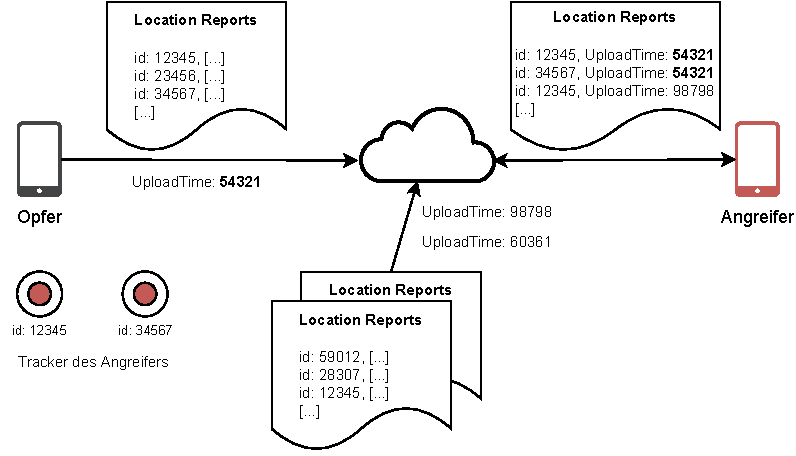
\includegraphics[width=0.9\textwidth]{indirektes_tracking.pdf}
  \caption{Schema zum indirekten Tracking von Personen.}
  \label{fig:indirect_tracking}
\end{figure}

Zur Nutzung als Tool für das Crowd-Monitoring werden einzelne Tracker an öffentlichen Orten platziert.
Finder Devices, die sich in der Nähe dieser Tracker befinden, generieren Location Reports und laden diese hoch.
Diese Reports können von Apples Servern heruntergeladen werden und erlauben Rückschlüsse über die Anzahl der iPhone-Nutzer, welche sich zu einem bestimmten Zeitpunkt in der Nähe eines Ortes aufgehalten haben.
Dazu werden die Erstellungszeitpunkte der Reports und die Anzahl der Reports für einen bestimmten Tracker herangezogen.
Die Zahl der iPhone-Nutzer kann weiterhin verwendet werden, um die Gesamtzahl der Personen zu schätzen.
Durch die Verzögerung beim Upload der Reports sind die Daten allerdings nur mit einer gewissen Verzögerung verfügbar \cite{Tonetto_FindMy}.

Über die Verwendung mehrerer Tracker lassen sich weiterhin die Bewegungen von Menschenmengen, der sogenannte Crowd-Flow, rekonstruieren.
Dabei werden die Tracker an verschiedenen Orten platziert und die Location Reports der Finder Devices heruntergeladen.
Anhand der Uploadzeitpunkte der Reports kann bestimmt werden, welche Reports vom gleichen Finder Device stammen \cite{Tonetto_FindMy}.
Darauf aufbauend kann die Zeit bestimmt werden, die das Finder Device benötigt hat, die Distanz zwischen jeweils zwei Trackern zurückzulegen.
Alternativ könnte, über das oben vorgestellte Verfahren, die Anzahl der Personen in der Nähe jedes Trackers zu verschiedenen Zeiten bestimmt werden und auf Basis der Veränderungen Rückschlüsse auf die Bewegungen der Menschenmengen gezogen werden.


Dieser Missbrauch des „Wo ist?“ Dienstes kann als Alternative zu aktuellen Crowd-Monitoring-Systemen, welche auf Bilderkennung oder der Auswertung von Wi-Fi Management Frames basieren, verwendet werden und erlaubt eine ähnliche Genauigkeit bei geringerem Eingriff in die Privatsphäre der betroffenen Personen.
Zusätzlich ist dieser Ansatz besser für die Privatsphäre der Betroffenen, da keine personenbezogenen Daten erhoben werden \cite{Tonetto_FindMy}.
Deshalb wird dieser Einsatzzweck als „positiver“ Missbrauch des „Wo ist?“ Dienstes bewertet.


\subsubsection{Gegenmaßnahmen}
Da hier sowohl positive als auch negative Einsatzzwecke möglich sind, sind Gegenmaßnahmen wünschenswert, welche den positiven Nutzen erhalten und gleichzeitig die mögliche negative Nutzung verhindern.
Der negative Missbrauch durch indirektes Tracking beruht darauf, Location Reports eines Finder Devices miteinander in Verbindung zu bringen.
Dazu werden die Upload-Zeitstempel verwendet, die von Apples Servern beim Empfang gespeichert werden.
Tonetto \textit{et al.} \cite{Tonetto_FindMy} schlagen daher eine Reduktion der Genauigkeit der Zeitstempel oder deren komplette Abschaffung als Gegenmaßnahmen vor.
Alternativ kann auch der Upload der einzelnen Location Reports zufällig verteilt werden.
Konkret werden zufällige Zeitintervalle oder zufällige, seit der Erstellung zurückgelegte Distanzen vorgeschlagen.

Diese Maßnahmen sind geeignet, die Zuordnung mehrerer Location Reports zu einem Finder Device zumindest zu erschweren.
Damit steigt auch der Aufwand für die Rekonstruktion von Bewegungen und die indirekte Verfolgung von Personen.

Der positive Missbrauch zum Crowd-Monitoring wird durch diese Gegenmaßnahmen nicht komplett verhindert.
Insbesondere die Abschätzung von Personendichten ist nicht davon abhängig, mehrere Location Reports zu einem Gerät zuzuordnen.
Die Bestimmung des Crowd-Flows, nach der in \cite{Tonetto_FindMy} vorgestellten Methode, ist hingegen auf diese Zuordnung angewiesen.
Allerdings ließe sich der Crowd-Flow auch anhand der Veränderung der Personendichte über die Zeit abschätzen.
Die Genauigkeit dieser Alternativen Lösung ist mangels Untersuchung durch die Autoren nicht bekannt.
Die Bestimmung der Personendichte ist nur von der Möglichkeit Location Reports abzurufen abhängig.
Damit lassen sich kaum Gegenmaßnahmen treffen, welche nicht die Funktionsweise des Dienstes an sich beeinflussen.
Die Limitierung der zurückgegebenen Anzahl von Location Reports könnte diese Methode zwar erschweren, allerdings würde so vermutlich auch die Genauigkeit der Standortinformationen von tatsächlich verlorenen Geräten reduziert werden.

Die Nutzer können sich gegen positiven und negativen Missbrauch nur schwer schützen.
Durch regelmäßige Verbindung mit einem WLAN-Netzwerk wäre es möglich, die Zuordnung von Location Reports zu einem Gerät einzuschränken, da jeder Upload weniger Location Reports enthält.
Jedoch ist die Verbindung mit einem WLAN-Netzwerk nicht immer möglich und auch nicht immer gewünscht.
Sinnvolle Schutzmaßnahmen müssen demnach von Apple getroffen werden.


\subsection[M5]{M5: Verdeckter Datentransfer}
\label{missbrauch:5}
Tonetto \textit{et al.} \cite{Tonetto_FindMy} und Bräunlein \cite{braeunlein_sendmy} zeigen unabhängig voneinander, dass der „Wo ist?“ Dienst auch für einen verdeckten Datentransfer mit einer niedrigen Übertragungsrate ausgenutzt werden kann.
Dabei werden Finder Devices dazu genutzt, Daten an Apples Server zu übertragen, welche vom Angreifer heruntergeladen und dekodiert werden können.
Beide verwenden für das Senden der Daten inoffizielle Tracker, um die Daten in den Advertisements zu senden.
Der verdeckte Datentransfer kann dem Angreifermodell des Angreifers in der Nähe (A2 in \autoref{fig:adversary_models}) zugeordnet werden.
Allerdings muss das Angreifermodell um das Ziel eines kostenfreien und unentdeckten Datentransfers und der Möglichkeit die Location Reports über die \acp{API} des Diensts herunterzuladen erweitert werden.


Bräunlein \cite{braeunlein_sendmy} kodiert eine zu sendende Nachricht in den öffentlichen Schlüssel, der in Advertisement-Paketen übertragen wird.
Für jedes Bit der Nachricht wird ein 28 Byte langes Array, bestehend aus der Position des Bits in der Nachricht, einer ID des Senders und dem Wert des Bits generiert.
Anstatt einen öffentlichen Schlüssel im Advertisement zu senden, werden die so kodierten Daten für eine definierte Zeitspanne gesendet.
Danach wird der Prozess für das nächste Bit der Nachricht wiederholt.
Diese Kodierung ist in \autoref{fig:sendmy_encoding} schematisch dargestellt.
\begin{figure}[ht]
  \centering
  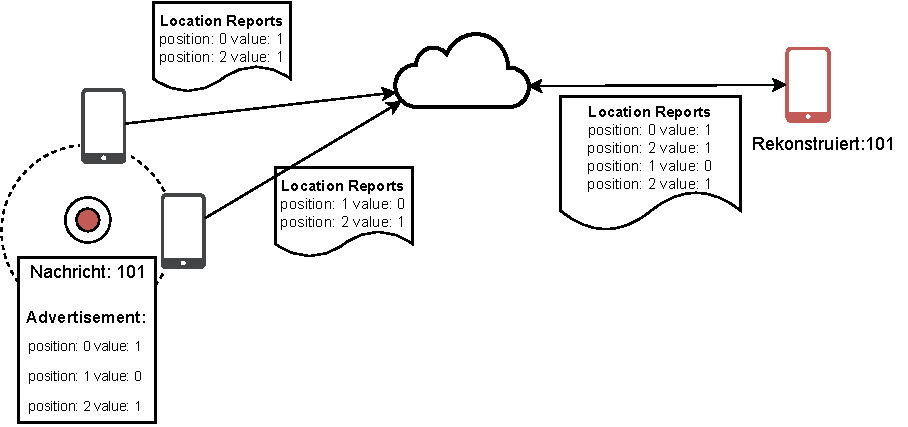
\includegraphics[width=0.95\textwidth]{sendmy.pdf}
  \caption{Bitweise Kodierung einer Nachricht in Advertisement-Pakete, wie von Bräunlein vorgeschlagen.}
  \label{fig:sendmy_encoding}
\end{figure}
Der Empfänger kann für jedes Bit der Nachricht die zwei möglichen Arrays generieren und eine Anfrage mit den jeweiligen \ac{SHA}-256 Hashes an Apples Server senden.
Da jedoch nur ein öffentlicher Schlüssel erzeugt wird, können mit diesen Schlüsseln verschlüsselte Nachrichten nicht entschlüsselt werden.
Jedoch ist für diesen Missbrauch die Entschlüsselung der Daten nicht notwendig, da lediglich das Vorhandensein eines bestimmten Location Reports überprüft werden muss, um die Nachricht zu dekodieren.
Abhängig davon, welcher der beiden Hashes in der Antwort enthalten ist, kann der Empfänger das Bit der Nachricht bestimmen.
Dabei wird ausgenutzt, dass jedes Apple Gerät die verschlüsselten Location Reports für beliebige öffentliche Schlüssel herunterladen kann \cite{Heinrich_OpenHaystack,braeunlein_sendmy}.
Da die Location Reports Ende-zu-Ende verschlüsselt sind, wird dadurch die Vertraulichkeit nicht gefährdet.
Ein Nachteil bei diesem Verfahren ist, dass somit theoretisch jedes Apple-Gerät die Nachricht abrufen könnte.

\begin{figure}[ht]
  \centering
  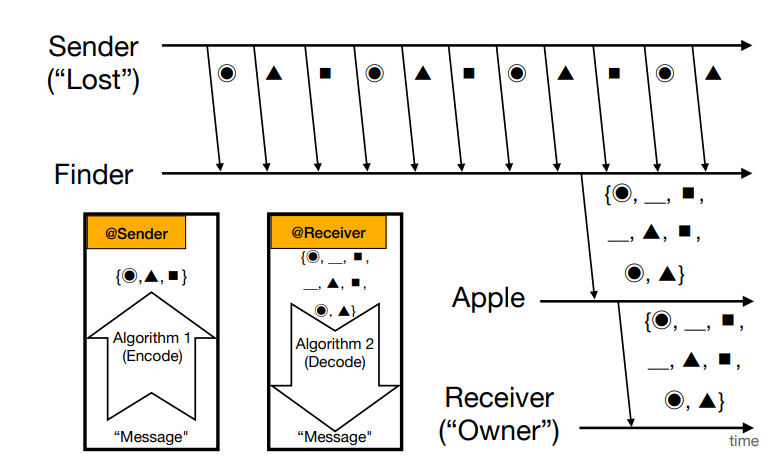
\includegraphics[width=0.7\textwidth]{tagcomm.png}
  \caption{Kodierung einer Nachricht in eine Folge bekannter Advertising Keys, wie von Tonetto \textit{et al.} vorgeschlagen \cite{Tonetto_FindMy}.}
  \label{fig:tagcomm_encoding}
\end{figure}
Das von Tonetto \textit{et al.} \cite{Tonetto_FindMy} vorgestellte Verfahren verwendet stattdessen 16 bekannte Advertising Keys, um die Nachricht in eine Folge dieser Keys zu kodieren.
Dazu wird eine Menge von Advertising Keys zuvor generiert und zwischen Sender und Empfänger ausgetauscht.
Das Verfahren ist in \autoref{fig:tagcomm_encoding} schematisch dargestellt.
Zunächst erzeugt der Sender aus der Nachricht eine Abfolge der Advertising Keys.
Diese werden in dieser Reihenfolge nacheinander in den Advertisement-Paketen gesendet.
Finder Devices, die sich in der Nähe befinden, empfangen die Advertisement-Pakete, erstellen Location Reports und laden diese hoch.
Der Empfänger der Nachricht kann alle Location Reports der bekannten Advertising Keys herunterladen.
Da der Empfänger die Location Reports entschlüsseln kann, erhält er die Zeitstempel der Erstellung der Location Reports.
Daraus kann er die Folge der Advertising Keys rekonstruieren und die Nachricht dekodieren.

Im Vergleich zum Verfahren von Bräunlein, werden hier echte Advertising Keys verwendet, sodass die Location Reports entschlüsselt werden können, sodass der Standort des Senders bestimmt werden kann.
Zusätzlich muss der Empfänger weniger Anfragen an Apples Server stellen, da nur 16 unterschiedliche Advertising Keys verwendet werden.
Bräunleins Verfahren benötigt hingegen zwei Anfragen an Apples Server pro übertragenem Bit \cite{braeunlein_sendmy}.


\subsubsection{Gegenmaßnahmen}
Der verdeckte Datentransfer über den „Wo ist?“ Dienst beeinträchtigt die Privatsphäre der Nutzer nicht.
Außerdem ist nur eine sehr geringe Datenrate möglich, was dieses Missbrauchsszenario für Angreifer in der Praxis weniger interessant macht.
Dennoch hat Apple ein berechtigtes Interesse, den kostenlosen Datentransfer über seinen Dienst zu verhindern.
Wie oben bereits beschrieben lässt sich dieser Missbrauch verhindern, indem die Nutzung von inoffiziellen Trackern unterbunden wird.

Weiterhin schlagen die Autoren von \cite{Tonetto_FindMy} vor, die Anzahl der Location Reports, die von einem Finder Device hochgeladen werden können, zu begrenzen.
Durch andere Finder Devices in der Nähe, reicht diese Begrenzung jedoch nicht aus um den verdeckten Datentransfer zu verhindern.
Zusätzlich könnte die Anzahl der abrufbaren Location Reports pro Advertising Key limitiert werden.
Die Kodierung, wie von Bräunlein \cite{braeunlein_sendmy} vorgeschlagen, wäre davon allerdings nicht betroffen, da für jedes Bit der Nachricht ein eigener Advertising Key verwendet wird.

Apple könnte zusätzlich den Abruf von Location Reports auf Lost Devices beschränken, die unter der gleichen Apple-ID registriert sind.
Eine Registrierung, welche die Zuordnung eines hochgeladenen Location Reports zu einer Apple-ID erlaubt, ist jedoch im Dienst aktuell nicht vorgesehen und würde eine signifikante Anpassung des Dienstes erfordern.
Entweder müsste der \ac{MBK} mit der Apple-ID verknüpft werden, was die Ende-zu-Ende-Verschlüsselung aufweicht, da Apple die Daten dann entschlüsseln könnte.
Alternativ müsste das Advertisement-Format um Daten zur Verknüpfung mit der Apple-ID erweitert werden.
Letzteres würde die Verfolgbarkeit von Lost Devices anhand der Advertisement-Pakete im Vergleich zum aktuellen System erleichtern.
Zusätzlich bietet bereits die aktuelle Implementierung keine Möglichkeit noch mehr Daten in einem einzelnen Advertisement-Paket zu senden.
Apple hat demnach keine Möglichkeit den Missbrauch einzuschränken, ohne signifikante Anpassungen des Dienstes vorzunehmen.
Da dieses Szenario die Privatsphäre der Nutzer nicht gefährdet wird auf die Erarbeitung möglicher Gegenmaßnahmen durch die Nutzer verzichtet.


\subsection[M6]{M6: Korrelation von Standorten durch Apple}
\label{missbrauch:6}

Das zweite Ziel im Angreifermodell des Dienstanbieters (A4 in \autoref{fig:adversary_models}) bezieht sich auf die Korrelation von Standorten mehrerer Nutzer.
Heinrich \textit{et al.} \cite{Heinrich_FindMy} zeigen, dass durch den authentifizierten Upload und Download, die Korrelation durch Apple theoretisch möglich ist.
Die konkreten Standorte können aufgrund der Ende-zu-Ende-Verschlüsselung nicht bestimmt werden.
Allerdings kann bestimmt werden, welches Gerät welche Location Reports erstellt und welcher Nutzer diese heruntergeladen hat.
Daraus lässt sich folgern, welche Nutzer sich zu welcher Zeit an einem gemeinsamen Ort aufgehalten haben.
Apple könnte diese Informationen für eigene Zwecke nutzen, zum Beispiel um soziale Beziehungen zwischen Nutzern für personalisierte Werbung zu analysieren.
In \cite{Heinrich_FindMy} wird zusätzlich gezeigt, dass diese Daten auch von Strafverfolgungsbehörden genutzt werden könnten, um beispielsweise die Identität von Demonstrationsteilnehmern zu bestimmen.

Zumindest nach US-Recht existieren verschiedene Möglichkeiten für Strafverfolgungsbehörden, von Apple gespeicherte Daten anzufragen \cite{Data_Access}.
In den „Richtlinien für Rechtsverfahren [für] Regierungs- und Strafverfolgungsbehörden außerhalb der USA“ \cite{Apple_FindMy_Data} gibt Apple an, dass aufgrund der Verschlüsselung kein Zugriff auf die Standortdaten der Nutzer möglich ist.
Allerdings stehen „Verbindungsprotokolle zu ‚Wo ist?’ [stehen] für einen Zeitraum von bis zu 25 Tagen zur Verfügung“ \cite{Apple_FindMy_Data}.
Um diese Verbindungsprotokolle zu erstellen, muss eine Zuordnung von Verbindungen zu Nutzern stattfinden.
Da Verbindungen zum „Wo ist?“ Dienst nur beim Upload oder Download von Location Reports entstehen, kann davon ausgegangen werden, dass Apple diese Daten speichert.
Mit den Daten zur Authentifizierung kann Apple alle Location Report zu bestimmten Nutzern zuordnen.
Das hier beschriebene Szenario ist dadurch auch praktisch umsetzbar und könnte bei entsprechendem Zugriff nicht nur von Apple, sondern auch von Strafverfolgungsbehörden genutzt werden.


\subsubsection{Gegenmaßnahmen}
Um die Korrelation der Standortdaten zu verhindern, muss entweder der Upload oder der Download der Location Reports ohne Authentifizierung erfolgen.
Ein nicht authentifizierter Upload würde jedoch den Upload gefälschter von Location Reports erleichtern, da dafür kein Apple-Gerät mehr benötigt würde.
Die Auswirkungen gefälschter Reports sind mit den Auswirkungen von Replay-Angriffen nach Szenario \nameref{missbrauch:1} vergleichbar und könnten die Verfügbarkeit und Integrität der Standortdaten gefährden.
Der Download könnte prinzipiell ohne Authentifizierung erfolgen, da die Location Reports Ende-zu-Ende-verschlüsselt sind und auch die aktuelle Implementierung nicht prüfen kann, ob ein Location Report zur Apple-ID gehört, die den Download anfordert.
Diese Maßnahme wird auch von Heinrich \textit{et al.} \cite{Heinrich_FindMy} vorgeschlagen.
Es wäre jedoch möglich, dass Gegenmaßnahmen für andere Missbrauchsszenarien, wie zum Beispiel \nameref{missbrauch:3} und \nameref{missbrauch:4}, einen authentifizierten Download erforderlich machen.
Weiterhin ist fraglich, inwieweit Apple ein Interesse daran hat, die Korrelation der Standorte der Nutzer zu verhindern.
Es ist aktuell nicht bekannt, ob Apple dieses Missbrauchsszenario für eigene Zwecke nutzt.
Auch ist nicht klar, ob und wie häufig Strafverfolgungsbehörden die Daten zu „Wo ist?“ anfragen, da diese Informationen in Apples Transparenzbericht nicht gesondert aufgeführt werden \cite{Apple_Transparency}.

Es sind weiterhin keine Maßnahmen bekannt, wie Nutzer diesen Missbrauch verhindern oder erschweren können.

%\input{sections/gegenmaßnahmen.tex}
\section{Fazit}
\label{sec:Fazit}

% \subsubsection{Acknowledgements} Please place your acknowledgments at
% the end of the paper, preceded by an unnumbered run-in heading (i.e.
% 3rd-level heading).

\bibliographystyle{splncs04}
\bibliography{sources}

\end{document}
